%!TEX encoding = UTF-8 Unicode
% !TeX spellcheck = en_GB

%%%%%%%%%%%%%%%%%%%%%%%%%%%%%%%%%%%%%%
\chapter{Models for $b \to s \ell \ell$ anomalies within MFV}\label{chap:flav}
%%%%%%%%%%%%%%%%%%%%%%%%%%%%%%%%%%%%%%
%%%%%%%%%%%%%%%%
%\section{Introduction}
%%%%%%%%%%%%%%%%
Recent results from $B$-factories including Belle and Babar as well as the LHCb-experiment involving the semileptonic decays of the beauty mesons $B^0, B^\pm,B_s \dots$ point to marked deviation of $ \sim 2.5 \sigma$ from the SM prediction, particularly in the branching fractions ratios
\begin{equation}
R_{K^{(*)}} \equiv {Br(B \to K^{(*)} \mu^{+} \mu^{-}) \over Br(B \to K^{(*)} e^{+} e^{-})},
\end{equation}
in the low dilepton mass bins ~\cite{Aaij:2014ora,Aaij:2017vbb,Aaij:2019wad,Abdesselam:2019wac,LHCb:2021trn}~\footnote{The data from the most recent measurement of the $R_{K^*}$~\cite{LHCb:2021trn} has not been used in this work, as the fits shown in this chapter predates these results.}. In addition to the results of angular analysis of the decay~$B \to K^{*} \mu^{+} \mu^{-}$~\cite{Descotes-Genon:2013wba,Descotes-Genon:2015uva}, with the observable $P_5^\prime$  showing similar deviation from the SM, the most recent measurement was published by LHCb~\cite{LHCb:2020lmf} if the light cone sum rules for modelling  the hadronic effects are considered. Other observables derived from the branching fractions of semileptonic and full leptonic final states of $B$ mesons decays, e.g. $ B_{s} \to e^{+} e^{-}$ also showed deviations from the SM with the $2\sigma-3\sigma$ range ~\cite{Chatrchyan:2013bka,Aaij:2017vad,Aaboud:2018mst,Aaij:2020nol}. These observables have in common the FCNC transition $ b \to s \ell \ell\, \, \ell = e, \mu$, and are in conflict with the SM lepton universality of EW couplings. This tension could be translated into a strong case for the evidence of BSM physics with lepton flavour universality violation~(LUV)~\cite{Hiller:2014yaa,Hiller:2014ula,Bordone:2016gaq}.\\
When these aberrant results are added to the recent muon anomalous magnetic moment $g-2$ measurement by Fermilab~\cite{Muong-2:2021ojo} or measurements of differential dilepton branching fractions of $B$-mesons,  grounds for the muons being the source of LUV are established, i.e.  the NP degrees of freedom contain muon-flavoured couplings.  However, the hadronic contributions  in the decay amplitudes and~$g-2$ corrections~\cite{Khodjamirian:2010vf,Lyon:2014hpa,Chobanova:2017ghn,Blake:2017fyh,Bobeth:2017vxj}, that require non-perturbative QCD~\cite{Jager:2014rwa,Ciuchini:2015qxb,Arbey:2018ics,Chrzaszcz:2018yza}, make such a conclusion debatable, see, e.g.~\cite{Ciuchini:2018anp,Hurth:2020rzx} and the most recent analysis, with the updated lepton flavour universality tests~\cite{Ciuchini:2021smi}. \\
Another class of $B$ decays involving the tree-level $ b \to c \tau \nu_\tau$ transitions has shown similar tension with the SM~\cite{Azatov:2018knx,Alok:2019uqc,Murgui:2019czp,Shi:2019gxi}. Amongst other, the observable $R_{D^{(*)}} \equiv Br(B \to D^{(*)} \tau \nu) / Br(B \to D^{(*)} \ell \nu)$, originally found at Babar~\cite{Lees:2013uzd} and subsequently measured at Belle~\cite{Huschle:2015rga} and LHCb~\cite{Aaij:2017uff} has shown a $\sim 20\%$ deviation from the SM. All of the anomalous flavour observables as summarised in~\autoref{fig:pull} with their pull in $\sigma$'s shown in blue,  compared the standard model predictions with their uncertainties in orange. \\
 \begin{figure}[ht!]
 	\centering
 	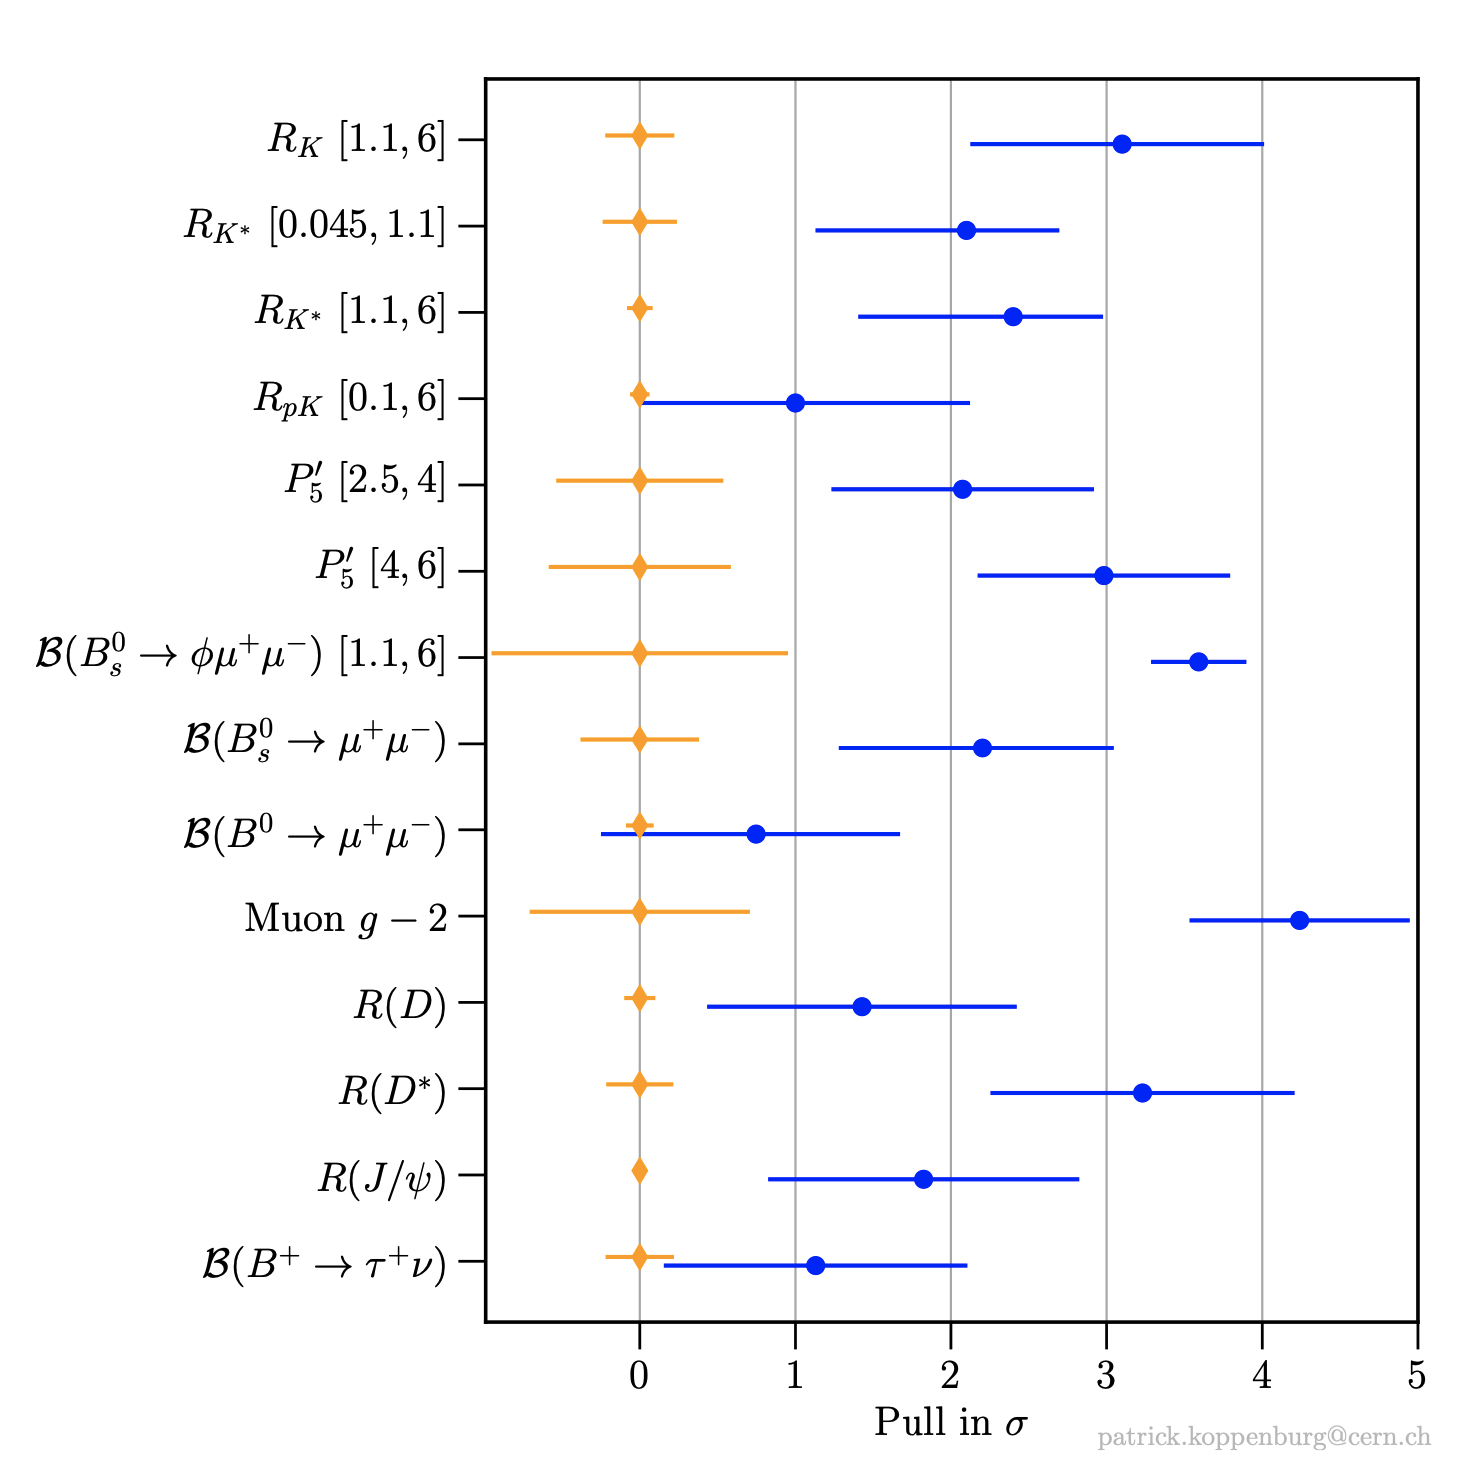
\includegraphics[width=0.65\textwidth]{fig/pull}
 	\caption{ Forest plot summarising the flavour observables in tension with the SM predictions, the experimental pull in terms of standard deviations $\sigma$ is shown in blue, while the SM prediction with the theoretical uncertainties is highlighted in orange. This figure is made by P.~Koppenburg~\cite{Koppenburg:2767155}. }
 	\label{fig:pull}
 \end{figure}
The simultaneous resolution for the anomalies emerging from $ b \to s \ell \ell$ and the semileptonic $b \to c$ transitions, requires models with complicated flavour structure~\cite{DiLuzio:2017vat,Calibbi:2017qbu,Bordone:2017bld,Barbieri:2017tuq,Assad:2017iib,Heeck:2018ntp,Fornal:2018dqn,Crivellin:2018yvo,Crivellin:2019dwb,Bordone:2019uzc}, as such models need to accommodate for similar deviations from the SM for both classes albeit these two transitions occur at different orders in the SM. Such models are often being at the edge of flavour physics constraints~\cite{Bona:2007vi,Silvestrini:2018dos} and collider bounds~\cite{Greljo:2017vvb,Baker:2019sli}.
On the other hand, most up-to-date measurements of $R_{D^{(*)}}$ from the Belle collaboration~\cite{Hirose:2016wfn,Abdesselam:2019dgh} turns out to be in good agreement with the SM~\cite{Bigi:2016mdz,Bernlochner:2017jka,Bigi:2017jbd,Jaiswal:2017rve}, thereby casting some doubt on the potential for NP lurking within $b\to c$ transitions. 
Furthermore, the ratios of branching fractions of decays involving the FCNC $b \to s \ell \ell$ transitions have a much lower dependence on the  non-perturbative QCD effects, that $g-2$, and differential distributions of semileptonic $B$-decays~\cite{Capdevila:2016ivx,Serra:2016ivr,Wehle:2016yoi,Alguero:2019pjc} . Therefore, the LUV information extracted from such ``clean'' observables have the highest potential for extracting LUV insights, see ~\cite{Kou:2018nap} for more details.\\
%%
The  $ b \to s \ell \ell$ anomalies have been studied in a model-independent manner, in particular SMEFT framework in refs.~\cite{DAmico:2017mtc,Geng:2017svp,Capdevila:2017bsm,Ciuchini:2017mik,Hiller:2017bzc} and more recently revisited in refs.~\cite{Ciuchini:2019usw,Aebischer:2019mlg,Alok:2019ufo,Alguero:2019ptt,Kowalska:2019ley,Arbey:2019duh,Datta:2019zca}.  Additionally, many UV-complete models were investigated, particularly leptoquarks~(LQ), like in~refs.~\cite{Calibbi:2015kma,Dorsner:2016wpm,Buttazzo:2017ixm,Kumar:2018kmr,Cornella:2019hct}. Another class of models of special interest are $Z^\prime$ models, in which the $B$ anomalies can be realised at loop-level. The simplest of these models has been proposed in ref.~\cite{Kamenik:2017tnu}, extending the SM with a single new $U(1)$ gauge group, together with the presence of top- and muon-partners, resulting in a top-philic $Z^\prime$ boson capable of evading present collider constraints~\cite{Fox:2018ldq} and responsible for the required LUV signatures. This model has the advantage of not introducing extra flavour spurions to the SM, i.e. similar to the MFV ansatz~\cite{Buras:2000dm,DAmbrosio:2002vsn,Kagan:2009bn}.  More general set of models with the same features can be found  in ref.~\cite{Celis:2017doq},  and subsequently elaborated upon in greater detail in the phenomenological study of ref.~\cite{Camargo-Molina:2018cwu}. \\
%%
While evading flavour constraints, models with top-philic $Z^\prime$ are in strong tension with the $Z$-pole measurements~\cite{Camargo-Molina:2018cwu,Efrati:2015eaa}. In fact, it has been shown in~\cite{Ciuchini:2019usw}, that in spite of  large hadronic uncertainties for the  amplitude of the $B \to K^{*} \mu^{+} \mu^{-}$ decay, a tension of at the 3$\sigma$ level at least would persist between $B$ data and EWPO for muonic LUV effects, and an even stronger tension would be found in the case of LUV scenarios involving electron couplings. This elucidates the interplay between $B$-physics and EWPO~\cite{Bhattacharya:2014wla,Feruglio:2016gvd,Celis:2017doq,Buttazzo:2017ixm,Kumar:2018kmr,Ciuchini:2019usw,Aebischer:2019mlg,Cornella:2019hct}. \\
%This fact has been brought to light recently~\cite{Coy:2019rfr} to abandon \textit{ii)}, and reformulate the original proposal addressing $B$ anomalies at one loop adding specific {BSM sources of flavour violation in order to reconcile $B$ data with EW precision tests in this context.} However, as briefly advertised in ref.~\cite{Ciuchini:2019usw}, an important caveat of this EW tension versus $B$ anomalies concerns the assumption of no tree-level NP contributions to EWPO. \\
%#########
This chapter aims to review a global fit including both EWPO and flavour observables related to the $B$-anomalies. Then present UV models that are based on ones present in the literature~\cite{Kamenik:2017tnu,Fox:2018ldq,Celis:2017doq},  that accommodate the resulting fit constraints are investigated. This work is an extension of several studies done by some of my collaborators~\cite{Ciuchini:2015qxb,Ciuchini:2016weo,Ciuchini:2017mik,Ciuchini:2017gva,Ciuchini:2018xll,Ciuchini:2018anp,Ciuchini:2019usw}, and published in~\cite{Alasfar:2020mne}. 
This chapter is organized as follows: in \autoref{sec:theory} , the SMEFT analysis of the flavour anomalies is presented; in \autoref{sec:UVtoymodels1} I discuss a viable $Z^{\prime}$ model in relation to our EFT results. After that, I present a possible alternative leptoquark scenarios in~in \autoref{sec:UVtoymodels2}. Lastly, the conclusions are summarised in \autoref{sec:sum}.
%%%%%%%%%%%%%%%%%%
\section{Flavour anomalies in SMEFT }
\label{sec:theory}
%%%%%%%%%%%%%%%%%%
\subsection{Theoretical preamble}
Global fits from $ b \to s \ell \ell$ anomalies show that  if NP degrees of freedom  enter at tree-level, they would have an energy scale $ \Lambda \sim 10$ TeV~\cite{DAmico:2017mtc,Geng:2017svp,Capdevila:2017bsm,Ciuchini:2017mik,Hiller:2017bzc}. Highlighting that for LHC phenomenology, the use of SMEFT is justified.  The operators of interest for the explanation of these $B$ anomalies are~\cite{Celis:2017doq,Ciuchini:2019usw,Aebischer:2019mlg}: 
\begin{eqnarray}
	\label{eq:tree_LUV_SMEFT}
	\mathcal{O}_{LQ^{(1)}}^{\ell \ell 23}, \,	(\mathcal{O}_{LQ}^{(1,3)})^{\ell \ell 23}, \, \mathcal{O}_{Qe}^{23 \ell \ell}, \,  \mathcal{O}_{Ld}^{ \ell \ell 23}, \, \mathcal{O}_{ed}^{\ell \ell 23 }.
\end{eqnarray}
Following the same convention for the SM fields in~\autoref{tab:thesm} and operator definitions in the Warsaw basis presented in~\autoref{warsaw}.  Current data, taking non-perturbative QCD effects into an account using light-cone sum rules, both left- and right-handed operators are permitted ~\cite{Ciuchini:2019usw,Alok:2019ufo,Alguero:2019ptt,Kowalska:2019ley}. Nevertheless, the statistical significance for the right-handed $b \to s$ interaction remains small, coming only from~$R_{K^{*}}/R_{K} \neq 1$ ~\cite{Hiller:2017bzc,Ciuchini:2019usw}. Hence, one can effective only consider the left-handed operators ~$(	\mathcal{O}_{LQ}^{(1,3)} )^{22 23}$ and~$\mathcal{O}_{Qe}^{23 22}$ for addressing the flavour anomalies. Additionally, when conservative hadronic uncertainties are considered ~\cite{Jager:2014rwa,Ciuchini:2015qxb,Arbey:2018ics}, the preference of NP coupling to the muons exclusively becomes mitigated and the inclusion of electron interactions becomes viable as well ~\cite{Ciuchini:2017mik}. From these considerations, we conclude that the operator ~$(	\mathcal{O}_{LQ}^{(1,3)} )^{\ell \ell 23}$ with either or both$ \ell=e, \mu$  offers the minimal resolution of these anomalies within the SMEFT framework~\cite{Ciuchini:2019usw}.\\
Introducing these operators at tree-level will lead to flavour violation beyond the SM, as these operators are flavour spurions unrelated to the SM ones. This can be avoided if they get generated at loop level from the RGE of operators involving the leptons and the Higgs~\cite{Celis:2017doq} 
\begin{eqnarray} 
	\label{eq:SMEFT_op_HL}
	(	\mathcal{O}_{\phi L}^{(1,3)})^{\ell \ell},	\,\,\, 	\mathcal{O}_{\phi e}^{\ell \ell},
\end{eqnarray}
or alternatively, from the semileptonic four-fermion (SL-4F) operators with right-handed top-quark currents:
\begin{eqnarray} 
	\label{eq:SMEFT_op_loop_lu}
		\mathcal{O}_{Lu}^{\ell \ell 3 3}, \,	\,\,	\mathcal{O}_{eu}^{\ell \ell 3 3} 
\end{eqnarray}
The leading log solution of the RGE for these operators ~\cite{Jenkins:2013zja,Jenkins:2013wua}, with the matching conditions for the left-handed quark-current operators in eq.~\eqref{eq:tree_LUV_SMEFT} at the  EW scale $\mu_{\textrm{\tiny{EW}}}\sim v $ are:\footnote{similar to the previous chapters, for one-loop effects,  the NP scale is set to be $\Lambda = 1$~TeV.  The renormalisation scale is set to $\mu_{\rm EW} = m_t\simeq v/\sqrt{2}$ to minimise the matching-scale dependence with the inclusion of the NLO	 corrections~\cite{Aebischer:2015fzz,Bobeth:2017xry}.}
\begin{eqnarray}
	\label{eq:SMEFT_matching_1loop}
	C_{LQ}^{(1)}\ ^{\ell \ell 23} &=& V_{ts}^{*} V^{ }_{tb} \left(\frac{y_{t} }{4 \pi}\right)^2 \log \left( \frac{\Lambda}{\mu_{\textrm{\tiny{EW}}}} \right)   \, \left(C_{Lu}^{\ell \ell 3 3} - C_{\phi L}^{(1)}\ ^{\ell \ell} \right)\,,\nonumber \\
		C_{LQ}^{(3)}\ ^{\ell \ell 23} &=& V_{ts}^{*} V^{ }_{tb} \left(\frac{y_{t} }{4 \pi}\right)^2 \log \left( \frac{\Lambda}{\mu_{\textrm{\tiny{EW}}}} \right)  \ C_{\phi L}^{(3)}\ ^{\ell \ell}  \,,\nonumber \\
	C_{Qe}^{23\ell \ell} &=& V_{ts}^{*} V^{ }_{tb} \left(\frac{y_{t} }{4 \pi}\right)^2 \log \left( \frac{\Lambda}{\mu_{\textrm{\tiny{EW}}}} \right)   \, \left( C_{eu}^{\ell \ell 3 3} - C^{\ell \ell}_{\phi e}\right) \, .
\end{eqnarray}
%%%%%%
In heavy quark physics, $B$ decays are typically studied within the low energy weak effective theory~\cite{Buchalla:1995vs,Buras:1998raa,Silvestrini:2019sey}, in which we have the vector and axial currents defined as
\begin{eqnarray}
	\label{eq:_Q9_Q10}
	\mathcal{O}_{9 V, \ell} & = & \frac{\alpha_{e}}{8 \pi} (\bar{s} \gamma_{\mu} (1-\gamma_{5})b) ( \bar{\ell} \gamma^{\mu} \ell ) \nonumber \ , \ \\
	\mathcal{O}_{10 A, \ell} & = & \frac{\alpha_{e}}{8 \pi} (\bar{s} \gamma_{\mu} (1-\gamma_{5})b) ( \bar{\ell} \gamma^{\mu} \gamma_{5} \ell ) \ ,
\end{eqnarray}
and matched at the EW scale $\mu_{\textrm{\tiny{EW}}}$  with the SMEFT operators in  eq.~\eqref{eq:SMEFT_op_HL}~-~\eqref{eq:SMEFT_op_loop_lu} follow:
\begin{eqnarray} 
	\label{eq:_C9_C10}
	C_{9,\ell}^{\rm NP}&=& \frac{\pi v^{2}}{\alpha \Lambda^2} \left(\frac{y_{t} }{4 \pi}\right)^2 \log \left( \frac{\Lambda}{\mu_{\textrm{\tiny{EW}}}} \right)   \, \left(C_{\phi L}^{(3)}\ ^{\ell \ell}-C_{\phi L}^{(1)}\ ^{\ell \ell}-C^{\ell \ell}_{\phi e}+ C_{Lu}^{\ell \ell 3 3} + C_{eu}^{\ell \ell 3 3} \right)\,,\nonumber \\
	C_{10,\ell}^{\rm NP}&=& \frac{\pi v^{2}}{\alpha \Lambda^2} \left(\frac{y_{t} }{4 \pi}\right)^2 \log \left( \frac{\Lambda}{\mu_{\textrm{\tiny{EW}}}} \right)   \, \left(C_{\phi L}^{(1)}\ ^{\ell \ell}-C_{\phi L}^{(1)}\ ^{\ell \ell}-C^{\ell \ell}_{\phi e}-s C_{Lu}^{\ell \ell 3 3} + C_{eu}^{\ell \ell 3 3} \right)\, .
\end{eqnarray} 
The overall normalization in the weak Hamiltonian follows the standard conventions adopted in refs.~\cite{Ciuchini:2015qxb,Ciuchini:2017mik,Ciuchini:2019usw}.
%%
As anticipated, the set of operators of interest for the study of $R_{K^{(*)}}$ in eq.~\eqref{eq:SMEFT_matching_1loop} is also sensitive to EWPO.  The operators involving the Higgs field and lepton bilinears in the SMEFT induce tree-level modifications to EW-boson couplings, while modifications of the $Z$ couplings to the leptons can be also induced via top-loop
 contribution~\cite{deBlas:2015aea}. In the leading-log approximation and at the leading order in the top Yukawa coupling, LUV effects can be generated by:
%
\begin{eqnarray}
	\label{eq:OLuedRGE}
	\left.\Delta g_{Z,L}^{\ell\ell}\right|_{\mathrm{LUV}} & = &
	- \frac 12 \left( C_{\phi L}^{(1)}\ ^{\ell \ell} +C_{\phi L}^{(3)}\ ^{\ell \ell} \right)\frac{v^2}{\Lambda^2}-
	3 \left( \frac{ y_t \, v}{4 \pi \Lambda} \right)^2 \log\left(\frac{\Lambda}{\mu_{\textrm{\tiny{EW}}}} \right) \, C_{Lu}^{\ell\ell33}  \ , \\ \nonumber
	\left.\Delta g_{Z,R}^{\ell\ell}\right|_{\mathrm{LUV}} & = & 
	- \frac 12 C^{\ell\ell}_{\phi e}\frac{v^2}{\Lambda^2}-
	3 \left( \frac{ y_t \, v}{4 \pi \Lambda} \right)^2 \log\left(\frac{\Lambda }{\mu_{\textrm{\tiny{EW}}}}\right) \, C_{eu}^{\ell\ell33} \ ,
\end{eqnarray}
where $\Delta g_{Z,L (R)}^{\ell\ell} \equiv g_{Z,L(R)}^{\ell\ell} - g_{Z,L (R)}^{\ell\ell,\textrm{SM}}$ is the deviation with respect to the left-handed (right-handed) leptonic couplings to the $Z$ boson in the SM theory. Since  EW couplings to leptons have been precisely measured at LEP/SLC, they provide an important test bed for lepton universality~\cite{Efrati:2015eaa,deBlas:2016ojx}.\\

These observations motivates a global SMEFT fit  of the operators explaining the  $B$-anomalies, as well as their interplay with EWPO.  Assuming that the LUV affects are generated by NP via radiative effects, matching what is see in  eq.~(\ref{eq:_C9_C10}). Consequently, the NP will contribute to EWPO at tree-level, whilst other SMEFT operators appearing from the REG mixing are assumed to be small or constrained from other processes.  In order for these assumptions to be fulfilled within SMEFT, the operators modifying the EW coupling of the quarks need to be included as well 
\begin{eqnarray} 
	\label{eq:SMEFT_op_HQ}
		\mathcal{O}_{\phi Q}^{(1)} \ ^{qq} , \,
		\mathcal{O}_{\phi Q}^{(3)}\ ^{qq} ,\,  
		\mathcal{O}_{\phi u}^{qq}, \, 
		\mathcal{O}_{\phi d}^{qq}, 
\end{eqnarray}
where $q=1,2,3$ identifies quark generations. These operators are considered to be flavour aligned, in a similar fashion to $C_{q\phi}$ of the previous chapter, in particular they are assumed to be aligned with the down-quark basis. This is needed to avoid pathological tree-level FCNC ~\cite{Silvestrini:2018dos}. The same holds for the leptonic operators, being aligned with the charged lepton mass bases.\\
%
The EWPO have a degeneracy between the first and second generation quarks, particularly in the down-type quarks sector. Therefore, it is natural to impose a $U(2)^3$ symmetry between first and second generator quark operators, thus imposing $C_{\phi Q}^{(1,3)}\ ^{11} = C_{\phi Q}^{(1,3)}\ ^{22} $, $C_{\phi u}^{11} = C_{\phi u}^{22}$. This also helps to suppress large FCNC contributions from these operators.  Additionally, the RGE boundary condition $C^{33}_{\phi u}=0$ is assumed. This is motivated by the fact that this Wilson coefficient cannot be constraint by EWPO, as modifications to $Z$-coupling to right-handed top quarks cannot be probed by by $Z$-pole measurements. 
Finally, for completeness, the four-lepton operator is also included in the fit:
\begin{equation}
	\label{eq:SMEFT_op_LLLL}
	O^{1221}_{LL}=(\bar{L}_1 \gamma^\mu L_2) (\bar{L}_2 \gamma_\mu L_1) \ ,
\end{equation}
which contributes to the muon decay amplitude, and therefore alters the extraction of the value of the Fermi constant, $G_F$, which is one of the inputs of the SM EW sector.

The operators in eqs.~\eqref{eq:SMEFT_op_HL}, \eqref{eq:SMEFT_op_HQ} and \eqref{eq:SMEFT_op_LLLL}, with the assumptions mentioned before, saturate all the 17 degrees of freedom, i.e. combinations of operators, that can be constrained in a fit to EWPO in the dimension-six SMEFT framework while keeping flavour changing neutral currents in the light quark sector under control. Together with the 4 four-fermion operators from eq.~\eqref{eq:SMEFT_op_loop_lu}, this completes a total of 21 operators, which is included in the fit setup described in the next section. 
%%%%%%%%%%%%%%%%%%
\section{Analysis technique}
\label{sec:strategy}
%%%%%%%%%%%%%%%%%%
%We now proceed to discuss in more detail our EFT analysis. {Our aim is to pin down the picture that should address the present $B$ anomalies via one-loop SM RGE effects of flavour-conserving dimension-six operators, and respect at the same time the constraints from EW precision.} We can achieve this goal with a comprehensive global analysis that aims at combining EWPO and $b \to s \ell \ell$ data.\footnote{See ref.~\cite{Capdevila:2020rrl} for another recent analysis where $b \to s \ell \ell$ data and EW measurements have been combined, with the different scope of resolving tensions in the determination of the Cabibbo angle~\cite{Belfatto:2019swo,Grossman:2019bzp}.}
The global fit combining both flavour observables related to the $ b \to s \ell \ell$ anomalies, in addition to EWPO is carried out in a Bayesian statistical framework. The experimental observables are modelled via state-of-the-art theoretical information already implemented and described in ref.~\cite{Ciuchini:2019usw} for flavour physics, and for EW and Higgs physics in ref.~\cite{Ciuchini:2013pca} and, more recently, in ref.~\cite{deBlas:2016ojx}. EWPO are extended by flavour non-universal  SMEFT contributions described in ref.~\cite{Efrati:2015eaa,deBlas:2019wgy}. The statistical and physics frameworks are both available within the publicly available \HEPfit~\cite{deBlas:2019okz} package, a Markov Chain Monte Carlo (MCMC) framework built using the Bayesian Analysis Toolkit~\cite{2009CoPhC.180.2197C}~\footnote{ \HEPfit is developed by some of my collaborators, who have co-authored this work}\\
The experimental input used for the global is summarised in the following, which are also implemented in \HEPfit code : 
\begin{itemize}
	\setlength\itemsep{0em}
	{\item The set of EWPO including the $Z$-pole measurements from LEP/SLD, the measurements of the $W$ properties at LEP-II, as well as several related inputs from the Tevatron and LHC measurements of the properties of the EW bosons~\cite{ALEPH:2005ab,Abe:2000uc,Group:2012gb,Schael:2013ita,Aaboud:2017svj,Khachatryan:2014iya,Abazov:2011ws}. The following lists the bulk of the EWPO included in the fits:
		%
		\begin{gather*}
			M_H,~m_t,~\alpha_S(M_Z),~\Delta \alpha_{\mathrm{had}}^{(5)}(M_Z),\\
			M_{Z},~\Gamma_{Z},~R_{e,\mu,\tau},~\sigma_{\mathrm{had}}, ~A^{e,\mu,\tau}_{FB},~A_{e,\mu,\tau},~A_{e,\tau}(P_\tau),~ R_{c,b},~A^{c,b}_{FB},~A_{s,c,b},~R_{u+c}, \\
			M_{W},\Gamma_{W},~\mathrm{BR}_{W\to e \nu,\mu \nu,\tau \nu},~\Gamma_{W\to cs}/\Gamma_{W\to ud+cs},~\left|V_{tb}\right|;
		\end{gather*}
		%
	}
	\item The angular distribution of $B\to K^{(*)}\ell^+\ell^-$ decays for both $\mu$ and $e$ final states in the large-recoil region.These include data from ATLAS~\cite{Aaboud:2018krd}, Belle~\cite{Wehle:2016yoi}, CMS~\cite{Khachatryan:2015isa,Sirunyan:2017dhj} and LHCb~\cite{Aaij:2015dea,Aaij:2020nrf}; in addition to the branching fractions from LHCb~\cite{Aaij:2016flj}, and of $B\to K^*\gamma$\footnote{NP effects from dipole operators are strongly constrained as extensively investigated in ref.~\cite{Paul:2016urs}. However, radiative exclusive $B$ decays still provide relevant information about hadronic effects~\cite{Ciuchini:2018anp}.} for which the HFLAV average is used~\cite{Amhis:2019ckw}; 
	\item Branching ratios for $B^{(+)} \to K^{(+)} \mu^+\mu^-$ decays in the large-recoil region measured by LHCb~\cite{Aaij:2014pli};
	\item The angular distribution of $B_s\to \phi\mu^+\mu^-$~\cite{Aaij:2015esa} and the branching ratio of  the decay $B_s\to\phi\gamma$~\cite{Aaij:2012ita}, measured by LHCb;
	\item The LUV ratios $R_K$~\cite{Aaij:2019wad} and $R_{K^*}$~\cite{Aaij:2017vbb} from LHCb and Belle~\cite{Abdesselam:2019wac};
	\item Branching ratio of $B_{(s)}\to \mu^+\mu^-$ measured by LHCb~\cite{Aaij:2017vad}, CMS~\cite{Chatrchyan:2013bka}, and ATLAS~\cite{Aaboud:2018mst}; we also use the upper limit on $B_s\to e^+e^-$ decay reported recently by LHCb~\cite{Aaij:2020nol}. 
\end{itemize}
The measurements of  $B\to K^{(*)}\ell^+\ell^-$ decays in the low di-lepton invariant mass region are plagued by large uncertainties for the charmonium resonance, and thus not included win the fit.  Moreover, the rare beauty baryonic decay $\Lambda_{b} \to  \Lambda \, \mu^{+} \mu^{-}$  is not considered as well. \\  Modelling the decays of hadrons involves factorisable (in terms of decay constant) and non-factorisable non-perturbative QCD effects. The non-factorisable effects emerge from long-distance hadronic contributions to~\cite{Khodjamirian:2010vf,Jager:2014rwa,Lyon:2014hpa} QCD loops appearing in radiative corrections to these decays. In this analysis, the  $B\to K^*\ell^+\ell^-$ has two different scenarios to describe these hadronic effects, discussed also in other previous works of my collaborators ~\cite{Ciuchini:2016weo,Ciuchini:2017mik,Ciuchini:2017gva,Ciuchini:2018xll,Ciuchini:2018anp,Ciuchini:2019usw}. The first is a conservative approach (Phenomenological Data Driven or PDD) as originally proposed in \cite{Ciuchini:2015qxb}, and refined in ref.~\cite{Ciuchini:2018anp}, whilst the second is a more optimistic one based on the results in~\cite{Khodjamirian:2010vf} (Phenomenological Model Driven or PMD). The PDD scenario is based on a generic model of the hadronic effects, which is simultaneously fitted to $b \to s \ell \ell$ data alongside the NP effects. Contrary to PDD approach, the PMD scenario the dispersion relations specified in~\cite{Khodjamirian:2010vf} is used constrain the hadronic contributions in the entire large-recoil region considered in the analysis, ergo PMD has smaller hadronic effects in the~$B\to K^*\ell^+\ell^-$ amplitudes~\cite{Ciuchini:2016weo}. Th choice of the hadronic uncertainties model significantly affects the outcome of the  fits to the $B$-decays observables~\cite{Ciuchini:2019usw}. \\ In order to be as general as possible, the SMEFT global fit is done for four different scenarios, described as follows:
\begin{itemize}
	\setlength\itemsep{0em}
	\item {\bf EW}: 
	Using EWPO data only with the assumptions discussed in~\autoref{sec:theory}. This fit includes the operators in eqs.~\eqref{eq:SMEFT_op_HL},~\eqref{eq:SMEFT_op_HQ}, and \eqref{eq:SMEFT_op_LLLL}, summing up to a total of 17 Wilson coefficients.
	%
	\item  {\bf EW (SL-4F Only)}: This refers to a fit done with the Wilson coefficients of the { SL-4F operators} involving the right-handed top current, reported in eq.~\eqref{eq:SMEFT_op_loop_lu}. This scenario incorporates the assumption that BSM enters the modifications of the $Z$ couplings to muons and electrons through top-quark loops only.
	%
	\item {\bf EW \& Flavour}: Wilson coefficients of all the { 21 operators} given in eq.~\eqref{eq:SMEFT_op_HL},~\eqref{eq:SMEFT_op_HQ}, and eq.~\eqref{eq:SMEFT_op_LLLL}, together with eq.~\eqref{eq:SMEFT_op_loop_lu} are varied.\\
   All of the EW data  as well as the flavour observables listed above are used. This scenario comes in two varieties, PDD and PMD, as explained above.
	\item {\bf Flavour}: These fits exclusively include the Wilson coefficients of the {\em 4 operators} (both electrons and muons) appearing in eq.~\eqref{eq:SMEFT_op_loop_lu}, and are done including only flavour data, i.e. excluding EW measurements. Results are again distinguished for the PDD and PMD cases. This fit is typically done when flavour anomalies are discussed in the literature. Hence, it was included here to emphasize the importance of including EWPO .
\end{itemize}


%%%%%%%%%%%%%%%%%%
\section{Results from the SMEFT}
\label{sec:EFT_results}
%%%%%%%%%%%%%%%%%%

%%%%%%%%%%%%%%%%%%
%\subsection[Analysis of EW and \texorpdfstring{$b \to s \ell \ell$}{b to s ll} data]
%{Analysis of EW and \boldmath$b \to s \ell \ell$ data}
%\label{sec:GEN_EFT_results}
%%%%%%%%%%%%%%%%%%
As a cross-check of the analysis code, the results of the EW fit produced ref.~\cite{Efrati:2015eaa} using \HEPfit were reproduced. 
The, these results were further expanded by the inclusion of the measurements and observables list in the {\bf EW} scenario introduced in the previous section, giving new constraints of the SMEFT Wilson coefficients involving of the operators with a Higgs-doublet current, also including loop effects under the hypotheses stated in \autoref{sec:theory}. The operators with leptonic currents produce non-universal couplings modifications between the leptons and the EW gauge bosons. Consequently, they also contribute though the RGE to the $B$- decays observables, as seen in eq.~\eqref{eq:SMEFT_matching_1loop}. The {\bf EW} fit results of these operators are plotted on the left panel of~\autoref{fig:ew_flav_bounds}, highlighted in orange. The error bars correspond to the 68\% CI bounds on these operators after marginalising the posterior distribution.  We observe compatibility with the SM within the 2$\sigma$ level. Note that EW data strongly correlate the operators under consideration among themselves, as can be seen in the correlation matrix presented in~\autoref{fig:ew_corr}.\\
\newpage
\begin{sidewaysfigure}[ht]
	\centering
	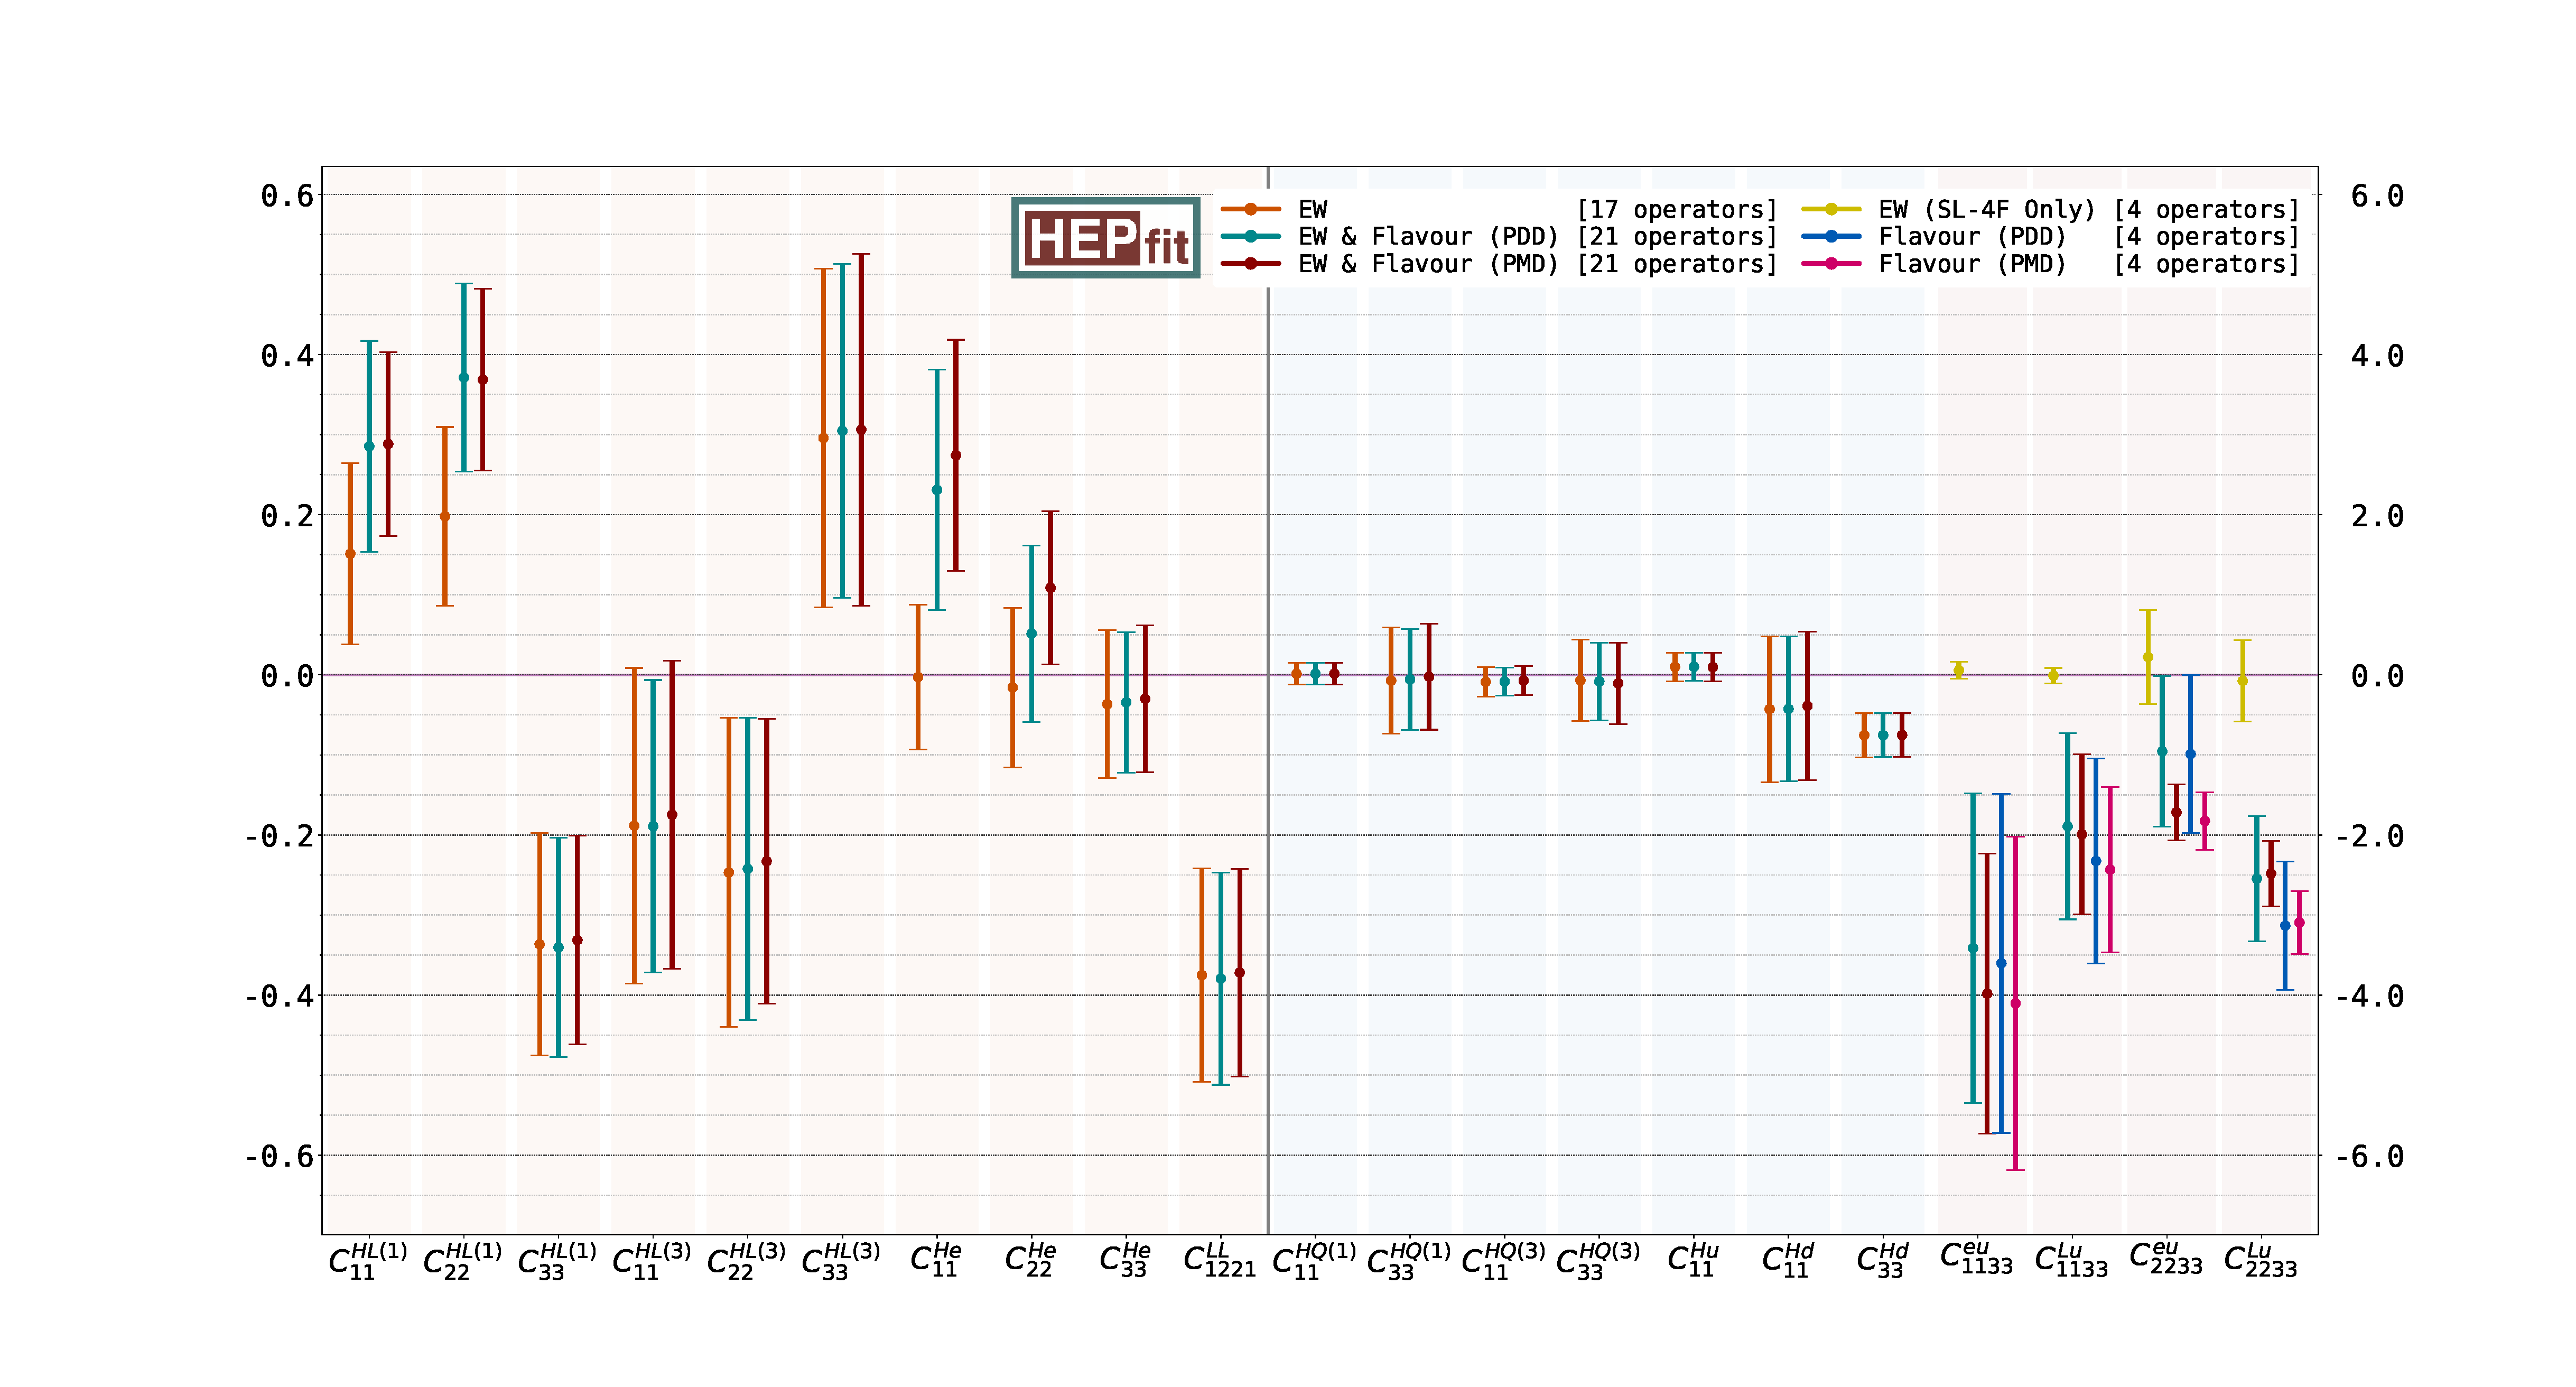
\includegraphics[width=\textwidth]{figures/errorbar.pdf}
	\caption{
		The marginalised fit results of the Wilson coefficients considered in the scenarios detailed in~\autoref{sec:strategy}. The central points denotes the mean of the marginalised posterior distribution, while the error bars are the 68\% CI constraint of the Wilson coefficients.  (Note the different scaling in the axes quantifying the size of the bounds presented in each half of the figure.) This figure is published in~\cite{Alasfar:2020mne}. 
	}
	\label{fig:ew_flav_bounds}
\end{sidewaysfigure}
\FloatBarrier
\begin{figure}[ht!]
	\centering
	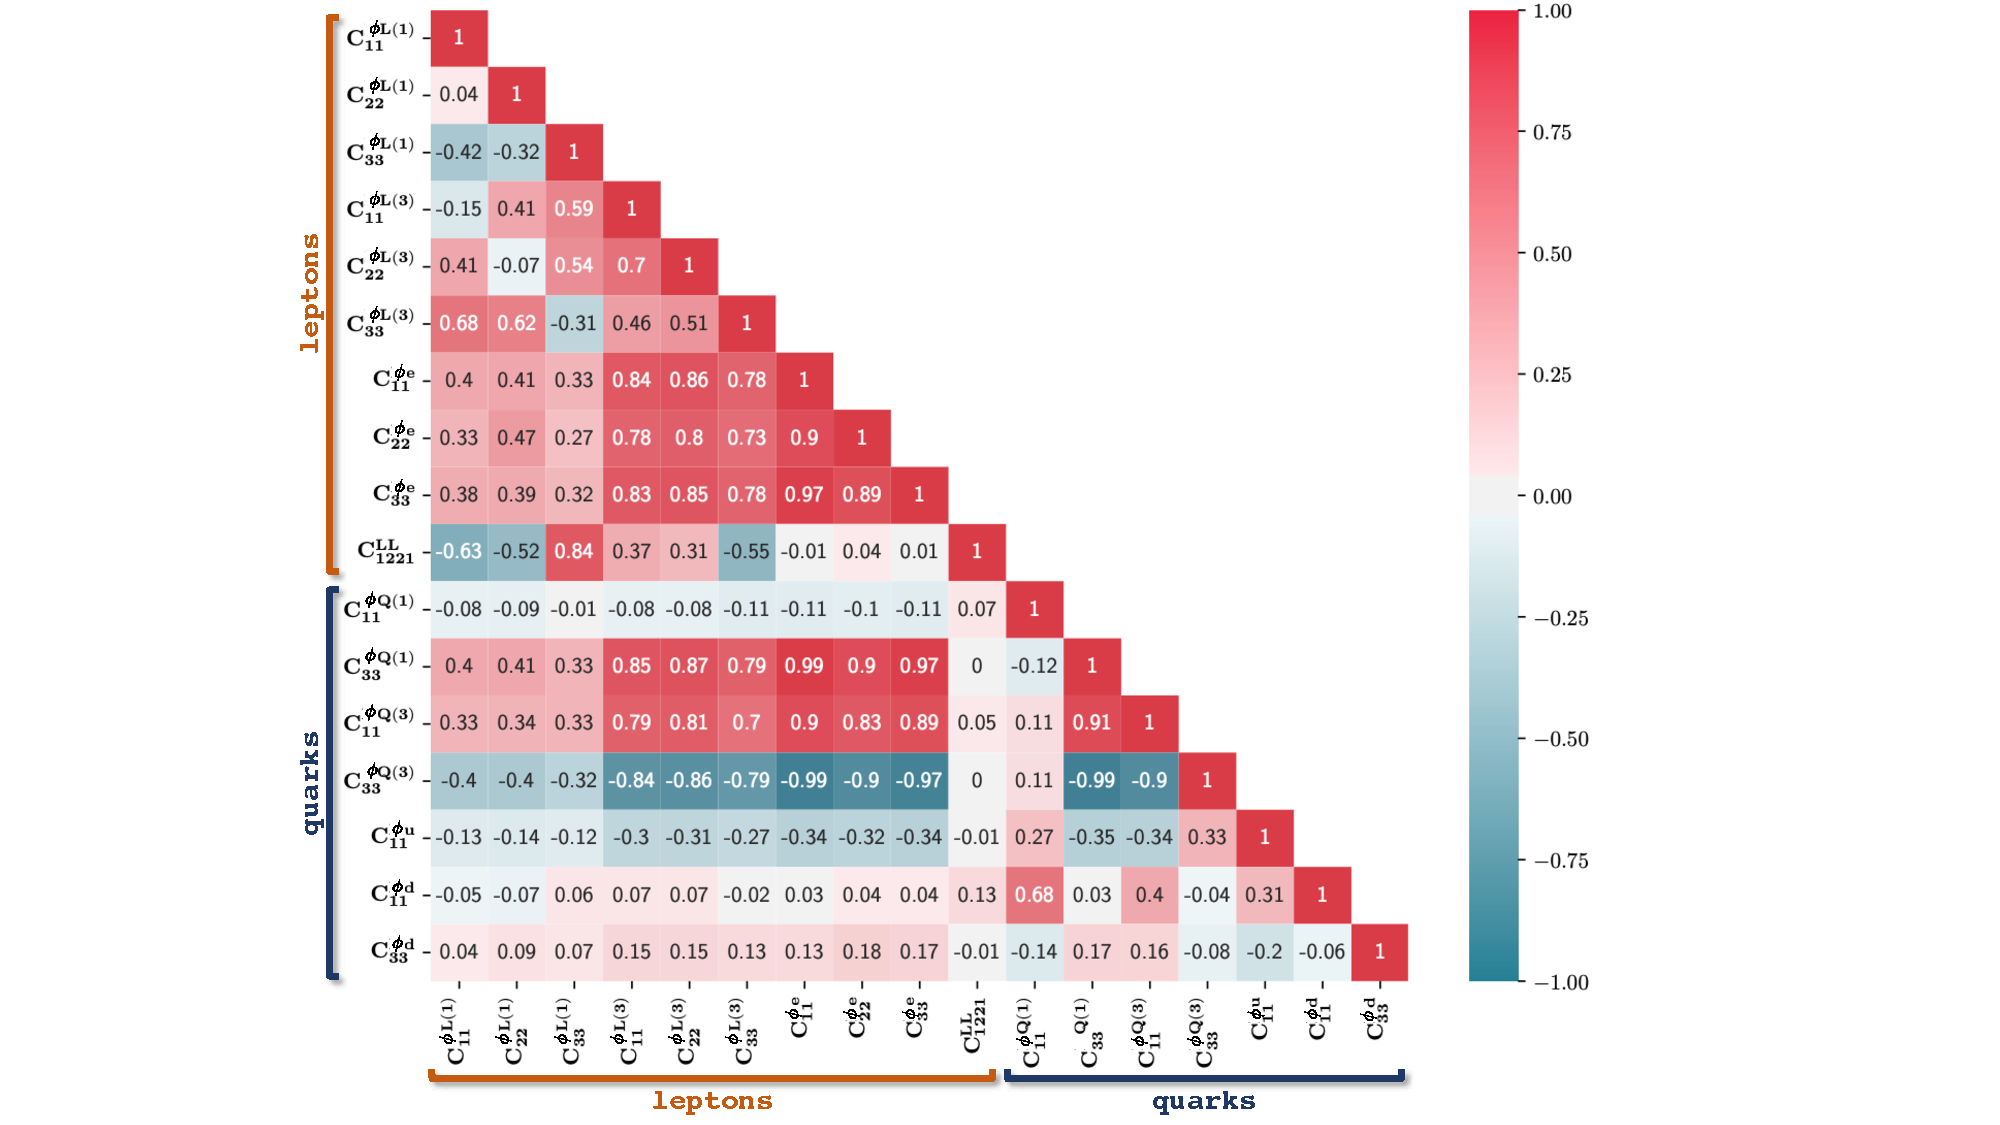
\includegraphics[width=\textwidth]{figures/heatmap_EW_loop.pdf}
	\caption{ The correlation matrix resulting from the Bayesian fit of the Wilson coefficient of the operators listed in in eqs.~\eqref{eq:SMEFT_op_HL}, \eqref{eq:SMEFT_op_HQ}, \eqref{eq:SMEFT_op_LLLL} in the \textbf{EW} scenario introduced in \autoref{sec:strategy}. The two distinct groups of Wilson coefficients associated to leptonic and quark interactions are remarked as ``leptons'' and ``quarks'', respectively. This figure is published in~\cite{Alasfar:2020mne}. }
	\label{fig:ew_corr}
\end{figure}
%\noindent where away from the photon pole, $R_{K^{(*)}}^{\textrm{\tiny SM}}$ are predicted to be unity at percent level~\cite{Bordone:2016gaq}.
\begin{figure}[htp!]
	\centering
	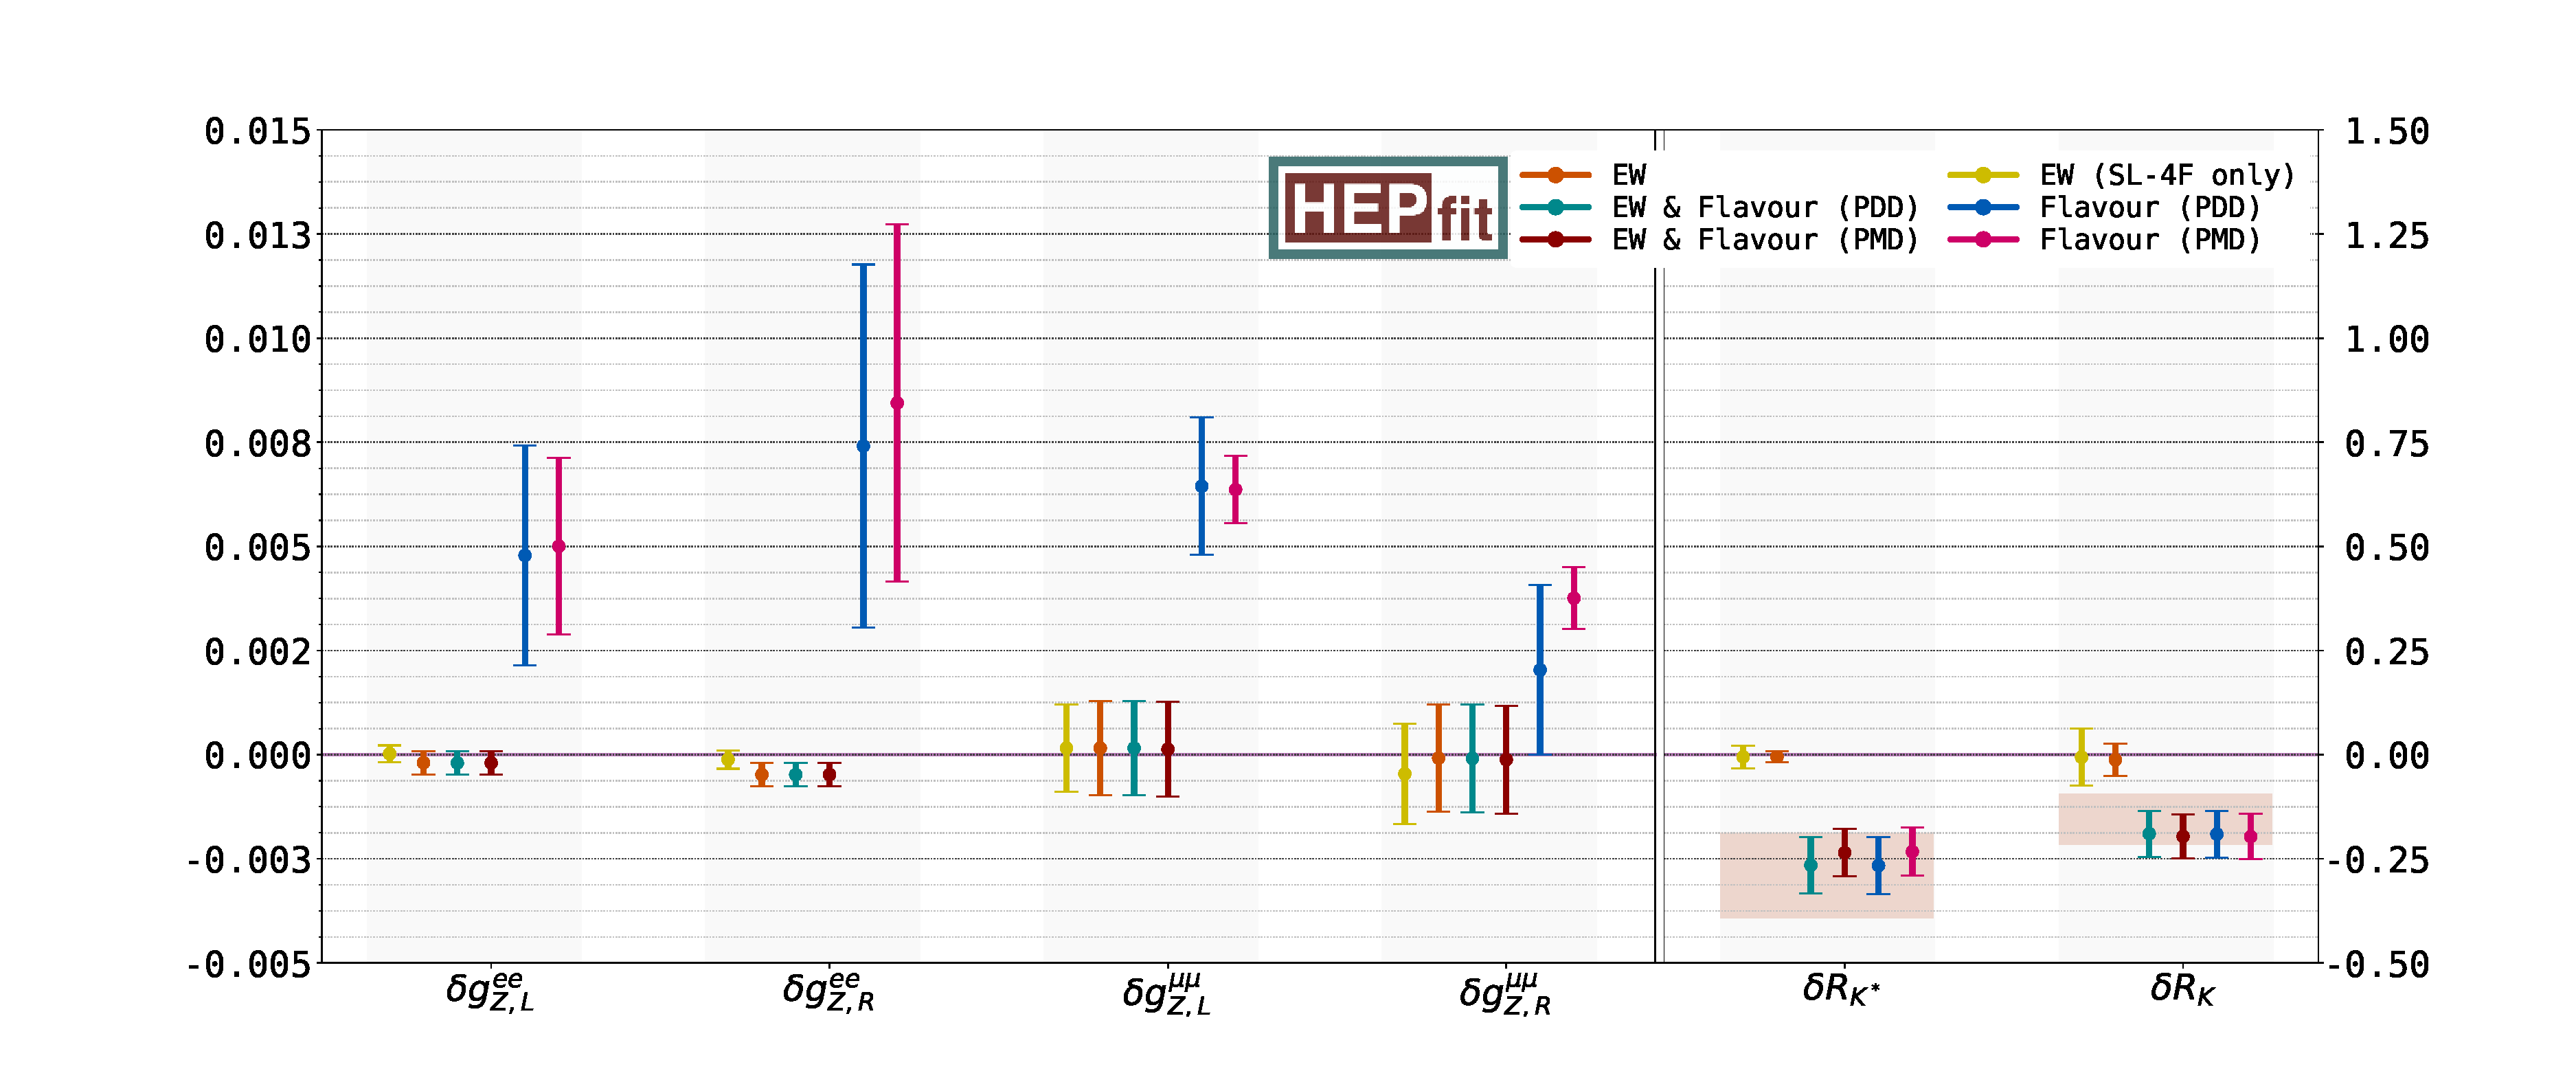
\includegraphics[width=\textwidth]{figures/errorbar_dg.pdf}
	\caption{ Fit results following the same convention as~\autoref{fig:ew_flav_bounds} for the $Z$ boson coupling modifiers for the muons and electrons, as well as the  lepton universality violating ratios, see eq.~\eqref{eq:SMdev}, with the red boxes indicating the region selected by the experimental measurements of $R_{K,(K^*)}$. This figure is published in~\cite{Alasfar:2020mne}. 
	}
	\label{fig:ew_flav_dg}
\end{figure}
Strong correlations can be observed between the Wilson coefficients from the leptonic and quark sectors, which are induced by the universal loop effects of the operator ${\cal O}_{\phi Q}^{(1)}\ ^{33}$ to all the EW couplings, as anticipated at the end of \autoref{sec:EFT_results}. 
This leads to a relaxation of the naive bounds on $C_{\phi L}^{(1)}\ ^{\ell\ell}$,$C_{\phi L}^{(3)}\ ^{\ell\ell}$ and $C_{\phi e}\ ^{\ell\ell}$ that one would obtain in a tree-level analysis.
The comparison between the tree-level fits and the ones presented in this section is presented in~\autoref{app:EW}. The results in \autoref{fig:ew_corr} can then be compared to those in \autoref{fig:ew_corr_tree} where, as it is apparent, there is a substantial decoupling between the dimension-six operators made of Higgs doublets and quark bilinears from the leptonic ones.
\begin{figure}[h!]
	\centering
	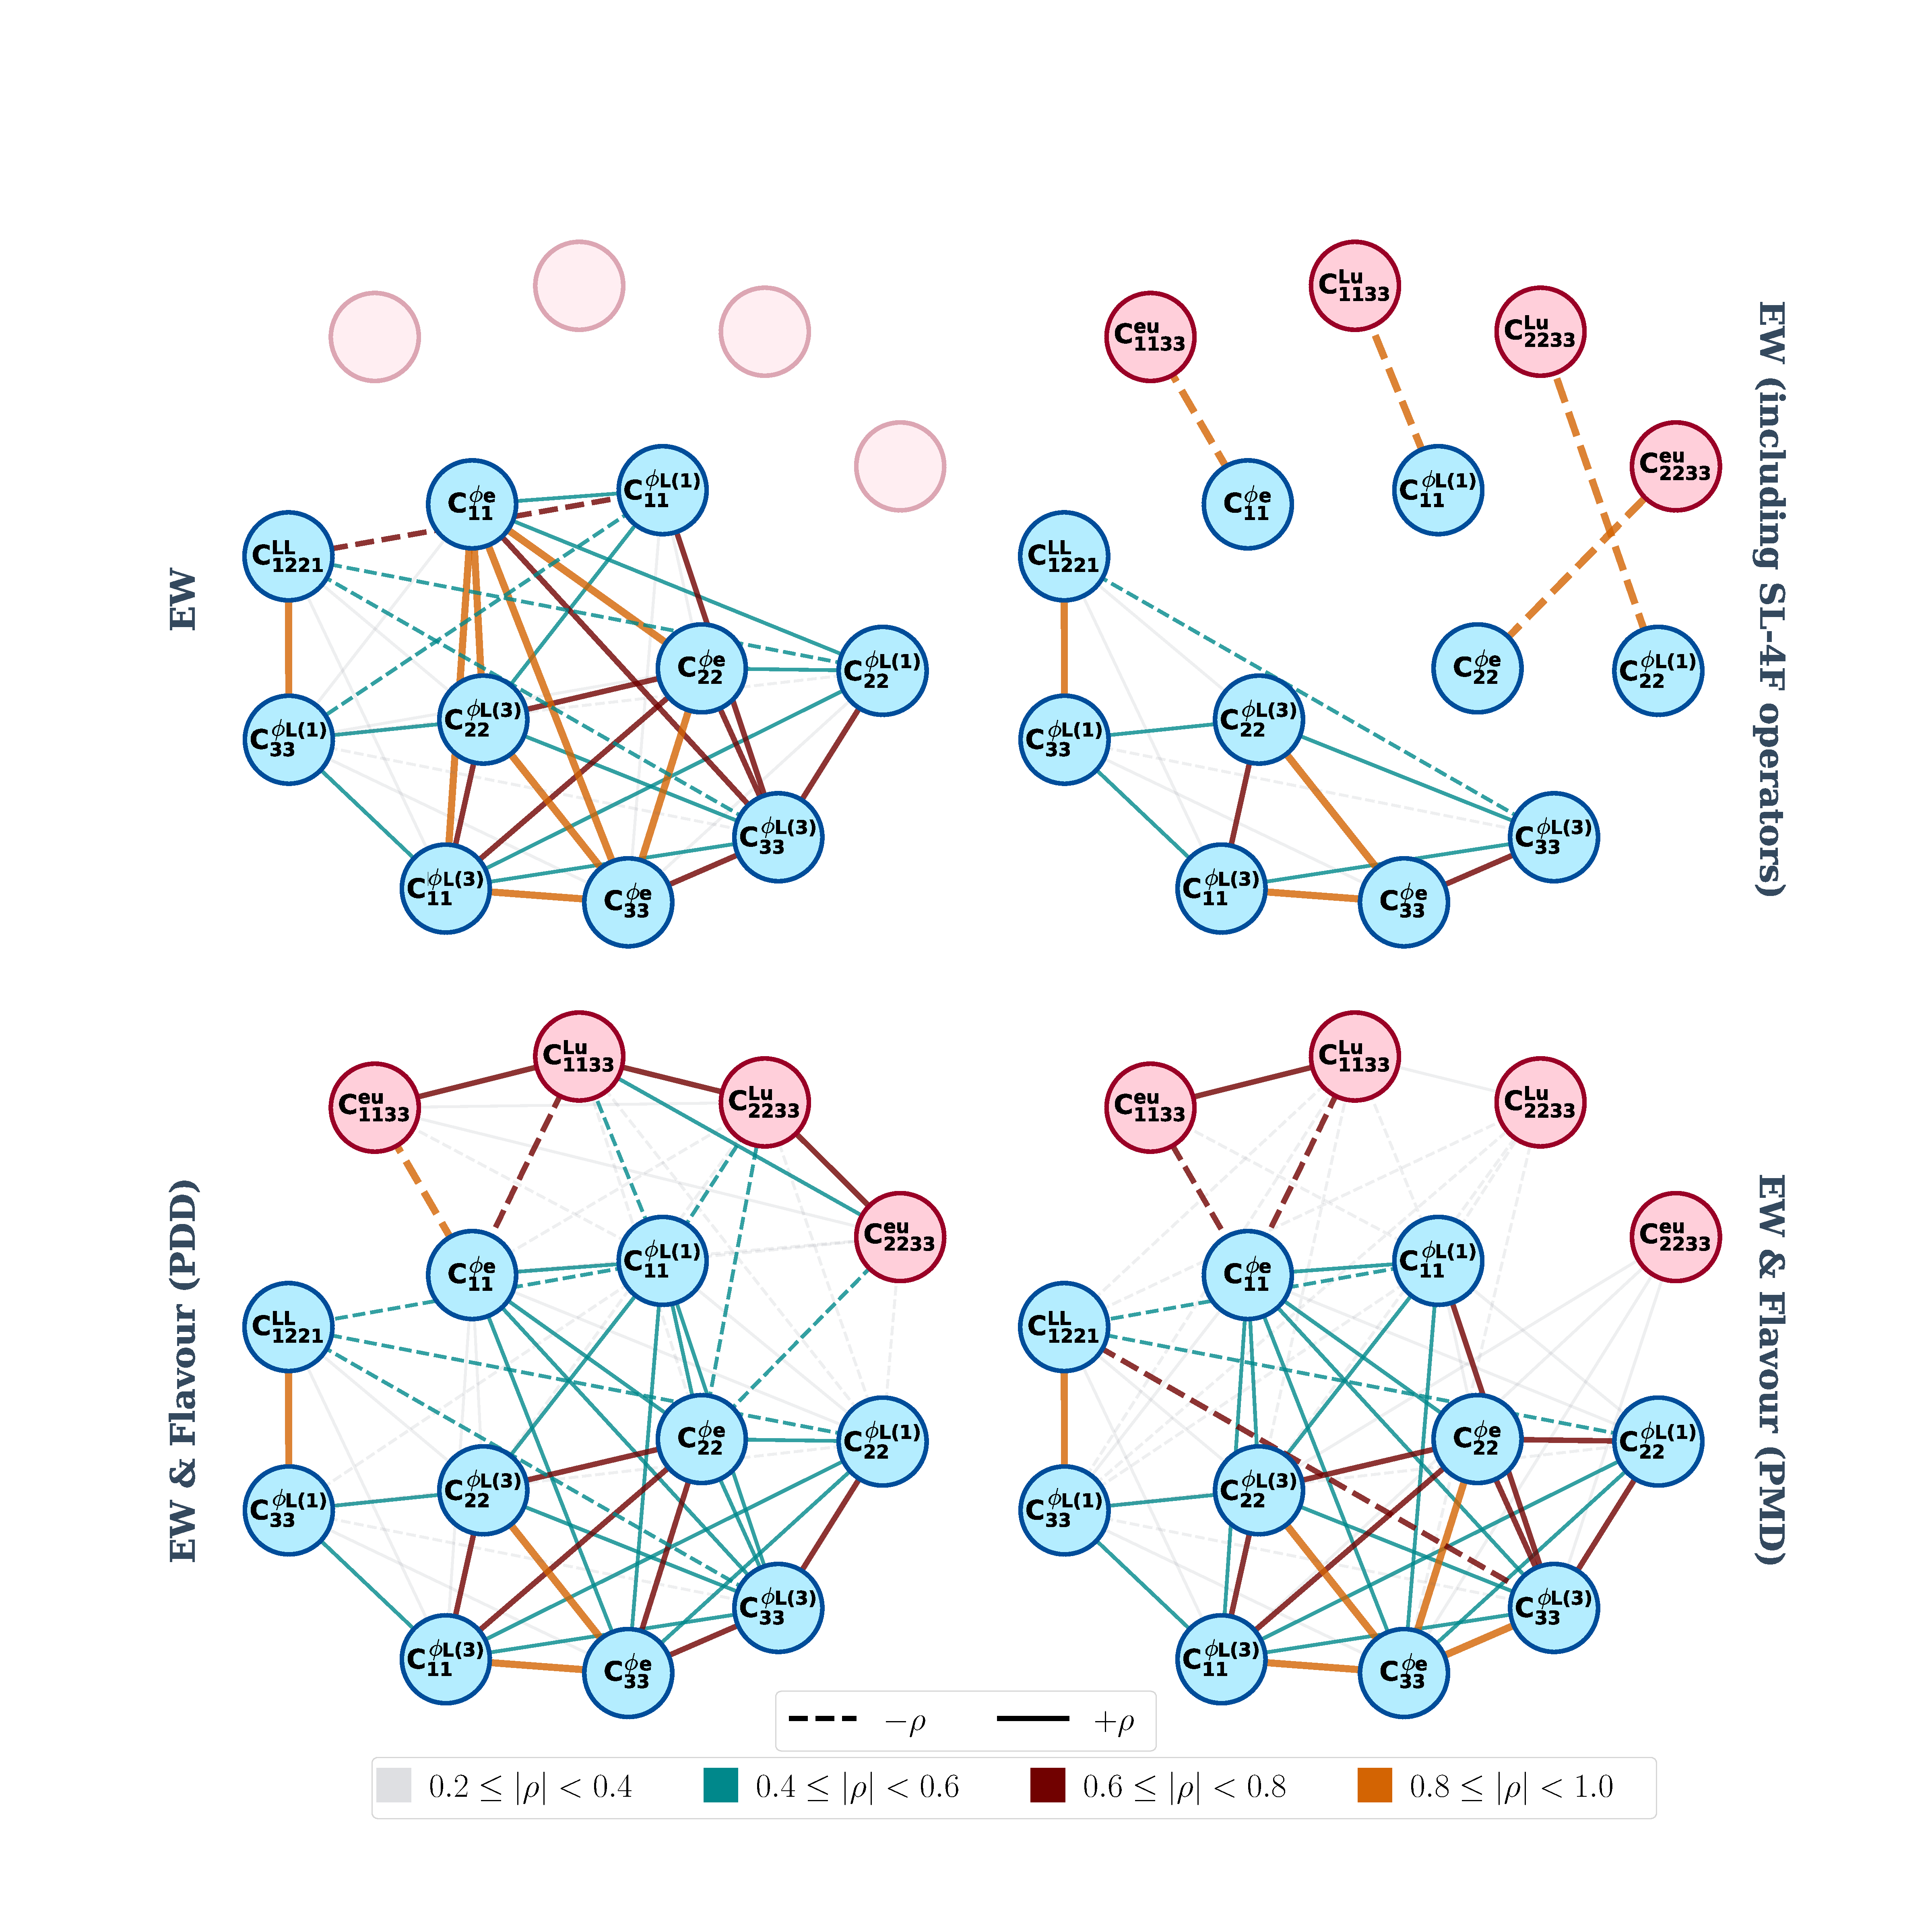
\includegraphics[width=0.9\textwidth]{figures/fixed_EW_flavour.pdf}
	\caption{ Network plot of the correlation between the Wilson coefficients considered in this study. The upper left panel shows the correlations from the \textbf{EW} fit , the upper right panel for the same fit but with the SL-4F Wilson coefficients included in the fit. The lower panel includes the flavour anomalies data  in the \textbf{EW+Flavour}  scenario, in which the degeneracy is broken. The lower left panel is for the PDD hadronic effects, while the lower right one is for the PMD case. This figure is published in~\cite{Alasfar:2020mne}. 
	}
	\label{fig:ew_flav_corr}
\end{figure}
The impact of these operators on the key observables for the present discussion is reported in \autoref{fig:ew_flav_dg}, where  it collects the mean and standard deviation on the shift in the $Z$ coupling to light leptons (normalized to the corresponding SM value),and on the effect on $R_{K^{(*)}}$ in the dilepton-mass range $[1.0,6.0]$~GeV$^2$: 
\begin{equation}
	\label{eq:SMdev}
	\delta g_{Z,L(R)}^{ee(\mu\mu)} \equiv g_{Z,L(R)}^{ee(\mu\mu)}{\big/}g_{Z,L(R)}^{ee(\mu\mu),\textrm{\tiny SM}}-1  \ , \ \delta R_{K^{(*)}} \equiv R_{K^{(*)}}^{ } - R_{K^{(*)}}^{\textrm{\tiny SM}} \ ,
\end{equation}
We can observe that that EW measurements tightly constrain NP effects modifying the $Z$-boson couplings to electrons, and also forbid deviations beyond the per-mille level in the case of couplings to muons. Therefore, the one-loop SMEFT contributions to $R_{K^{(*)}}$ are projected to be tiny. \\
The same conclusions can be derived when the fit is repeated for the  {\bf EW (SL-4F Only)} scenario, which is highlighted in yellow in \autoref{fig:ew_flav_bounds} and \autoref{fig:ew_flav_dg}. However, there is one exception, this scenario only allows for loop contributions to $\delta g_{Z,L(R)}^{\ell\ell}$ and $\delta R_{K^{(*)}}$ from  $C_{Lu,eu}^{\ell \ell 3 3}$ as depicted in eq.~\eqref{eq:SMdev}. This in turn allows for larger $b \to s  \ell \ell$ flavour observables  than the {\bf EW} scenario, see \autoref{fig:ew_flav_dg}. Though this does not affect the tension between the EWPO's and the experimental measurements of  $R_K$ and $R_{K^*}$ (indicated by the shaded red boxes in the right side of the figure) at the 3$\sigma$ level.\\
%%%
Moving on to the {\bf Flavour} scenario, using more recent flavour data, but effectively the same analysis strategy as ref.~\cite{Ciuchini:2019usw}. The fit results in the figures above for {\bf Flavour} scenario are highlighted in blue for the PDD and pink for PMD ans\"atze for the hadronic contributions. The fits favours non-zero $C_{Lu}^{2233}$ at more than 3$\sigma$ in the PDD case, and at roughly 6$\sigma$ in the PMD one. The main difference between these two ans\"atze stems from the results of the angular analysis of $B \to K^{*} \mu \mu$ decay. The PDD approach favours the fully left-handed NP coupling, i.e.  $C_{9, \ell} = - C_{10, \ell}$, and allows for NP coupling to electrons, while the PMD exclusively predicts the muonic resolution~\cite{Ciuchini:2017mik,Ciuchini:2019usw}. Looking at the flavour data fit results in \autoref{fig:ew_flav_dg}, we observe an apparent conflict between EWPO predictions of the $Z$ couplings and the $b \to s \ell \ell$ measurements. The inconsistency between the resolution of $B$ anomalies and EW data is exacerbated further for PMD case, where the tension between EWPO and $B$ anomalies  reaches up to $6\sigma$ for $g^{\mu \mu}_{Z,L}$. \\ 
Consensus between $b \to s \ell \ell$ measurements and EWPO can be reached in a true global fit manifesting in the {\bf EW \& Flavour}  scenario. This fit is shown in ref and green in the previously mentioned figures for the PDD and PMD cases, respectively. Revisiting  \autoref{fig:ew_flav_dg}, and looking at the red and green points for this fit  scenario, we observe that the $R_{K^{(*)}}$ anomalies are solved whilst EW precision being respected . Additionally,  this fit offers a new insight into this matter: it highlights strong correlations between the dimension-six operators $\mathcal{O}_{Lu(eu)}^{\ell\ell33}$ and $\mathcal{O}_{\phi L}^{(1)}\ ^{\ell\ell}/\mathcal{O}_{\phi e}^ {\ell\ell}$ as is evident from the network plot in\autoref{fig:ew_flav_corr}. This figure presents a pictorial representation of the correlations between the leptonic operators included in the different fits. \\
%\noindent Succinctly, an obvious solution which satisfies these constraints is a class of models where $R_{K^{(*)}}$ anomalies are addressed at tree level and where modifications to $Z$-lepton-lepton vertices are at the same time suppressed. However, these models would not offer a solution to $B$ anomalies of the MFV type envisaged so far, namely they would rely on the existence of sizeable new sources of flavour violation. 
Apart from the fits introduced in the previous section, for illustration purposes we also show in \autoref{fig:ew_flav_corr} the correlations obtained in a variant of the ${\bf EW}$ fit including also the four-fermion operators $O_{Lu(eu)}^{\ell\ell33}$, labelled as {\bf EW (including SL-4F operators)}. 
This is shown in the upper-right corner of the figure. As can be seen in that panel, and one could deduce from the relations in eq.~\eqref{eq:OLuedRGE}, in a pure EW fit adding the four-fermion operators would simply introduce 4 flat directions. These are illustrated by the links connecting the $C_{eu}^{\ell\ell 33}$ ($C_{Lu}^{\ell\ell 33}$) and $C_{\phi e}^{\ell\ell}$ ($C_{\phi L}^{(1)}\ ^{\ell\ell}$) operators, corresponding to 100\% anti-correlation.
Such flat directions are lifted upon the introduction of the flavour measurements of $R_{K}$ and $R_{K^*}$, as can be seen in the lower panels of \autoref{fig:ew_flav_corr} for the {\bf EW \& Flavour} fits.
%
Even then, due again to relations in eq.~\eqref{eq:SMEFT_matching_1loop} and~\eqref{eq:OLuedRGE} and the comparatively different precision of the EW and flavour measurements, sizeable correlations remain. 

%%
%In \autoref{fig:ew_flav_bounds} the imprint of these correlations is a shift of central values and an increase on the bounds on the corresponding Wilson coefficients, with red and green bars representing the outcome of the fit in the {\bf EW \& Flavour} scenario within the {\bf PMD} and {\bf PDD} approaches, respectively. The interplay between $O^{Lu(eu)}_{\ell\ell33}$ and $O^{HL^{(1)}(He)}_{\ell\ell}$ is evident when comparing the reported red and green bounds versus the orange EW constraints on $C^{HL^{(1)}(He)}_{\ell\ell}$, and the yellow ones for $C^{Lu(eu)}_{\ell\ell33}$. Consequently, as clearly depicted in \autoref{fig:ew_flav_dg}, looking at the red and green ranges reported for the {\bf EW \& Flavour} scenario, $R_{K^{(*)}}$ puzzles are solved with EW precision being respected. It is important to emphasize that, despite the significant correlation between quark and lepton operators introduced by the one-loop effects of $C_{33}^{HQ^{(1)}}$, quark operators play no significant role in reconciling the EWPO constraints with the solution to $B$ anomalies. This will become clearer in the next section, but can be easily understood from the fact that, as mentioned before, quark and lepton constraints are somewhat uncorrelated in the tree-level EW fit, and the fact that the one-loop corrections effect induced by $C_{33}^{HQ^{(1)}}$ are flavour universal.


%\subsection{A minimal EFT picture}
It is not necessary to invoke all of the 21 SMEFT operators considered in the {\bf EW \& Flavour} scenario in order to have a resolution for the flavour anomalies and EWPO. A simpler picture using two or four operator suffices to fulfil the experimental need to explain LUV and respect EW measurements. This picture contain the fully left-handed operator, $\mathcal{O}_{LQ}^{\ell \ell 2 3}$ and $\mathcal{O}_{\phi L}^{(1)} \ ^{\ell \ell}$. The former operator would be generated at a loop-level by $\mathcal{O}_{Lu}^{\ell \ell 3 3}$, while the latter at tree-level.  This minimalist SMEFT approach would then include only  $\mathcal{O}_{\phi L}^{(1)} \ ^{\ell \ell}$ and $\mathcal{O}_{Lu}^{\ell \ell 3 3}$, and $\ell= \mu, e$. So the model could involves either muons, electrons or both of them.\\ 
In~ \autoref{fig:2D_correlations}, the EWPO (grey), flavour with PDD (orange) and combined (magenta) fits for this minimal SMEFT model. For the muonic (left) and electronic (right) solutions. We observe that the tension between EWPO and $b \to s \ell \ell$ data if individual fits were preformed, whilst this is resolved in the combined fit. However, this induces correlation between the four-fermion operator $\mathcal{O}_{Lu}^{\ell \ell 3 3}$ and the one involving the Higgs-doublet and lepton bilinears. This model also obeys MFV assumptions, which protects it from other flavour observables. However, as mentioned earlier, the $B$ anomalies has to be explained at one-loop level. 
\begin{figure}[htpb!]
	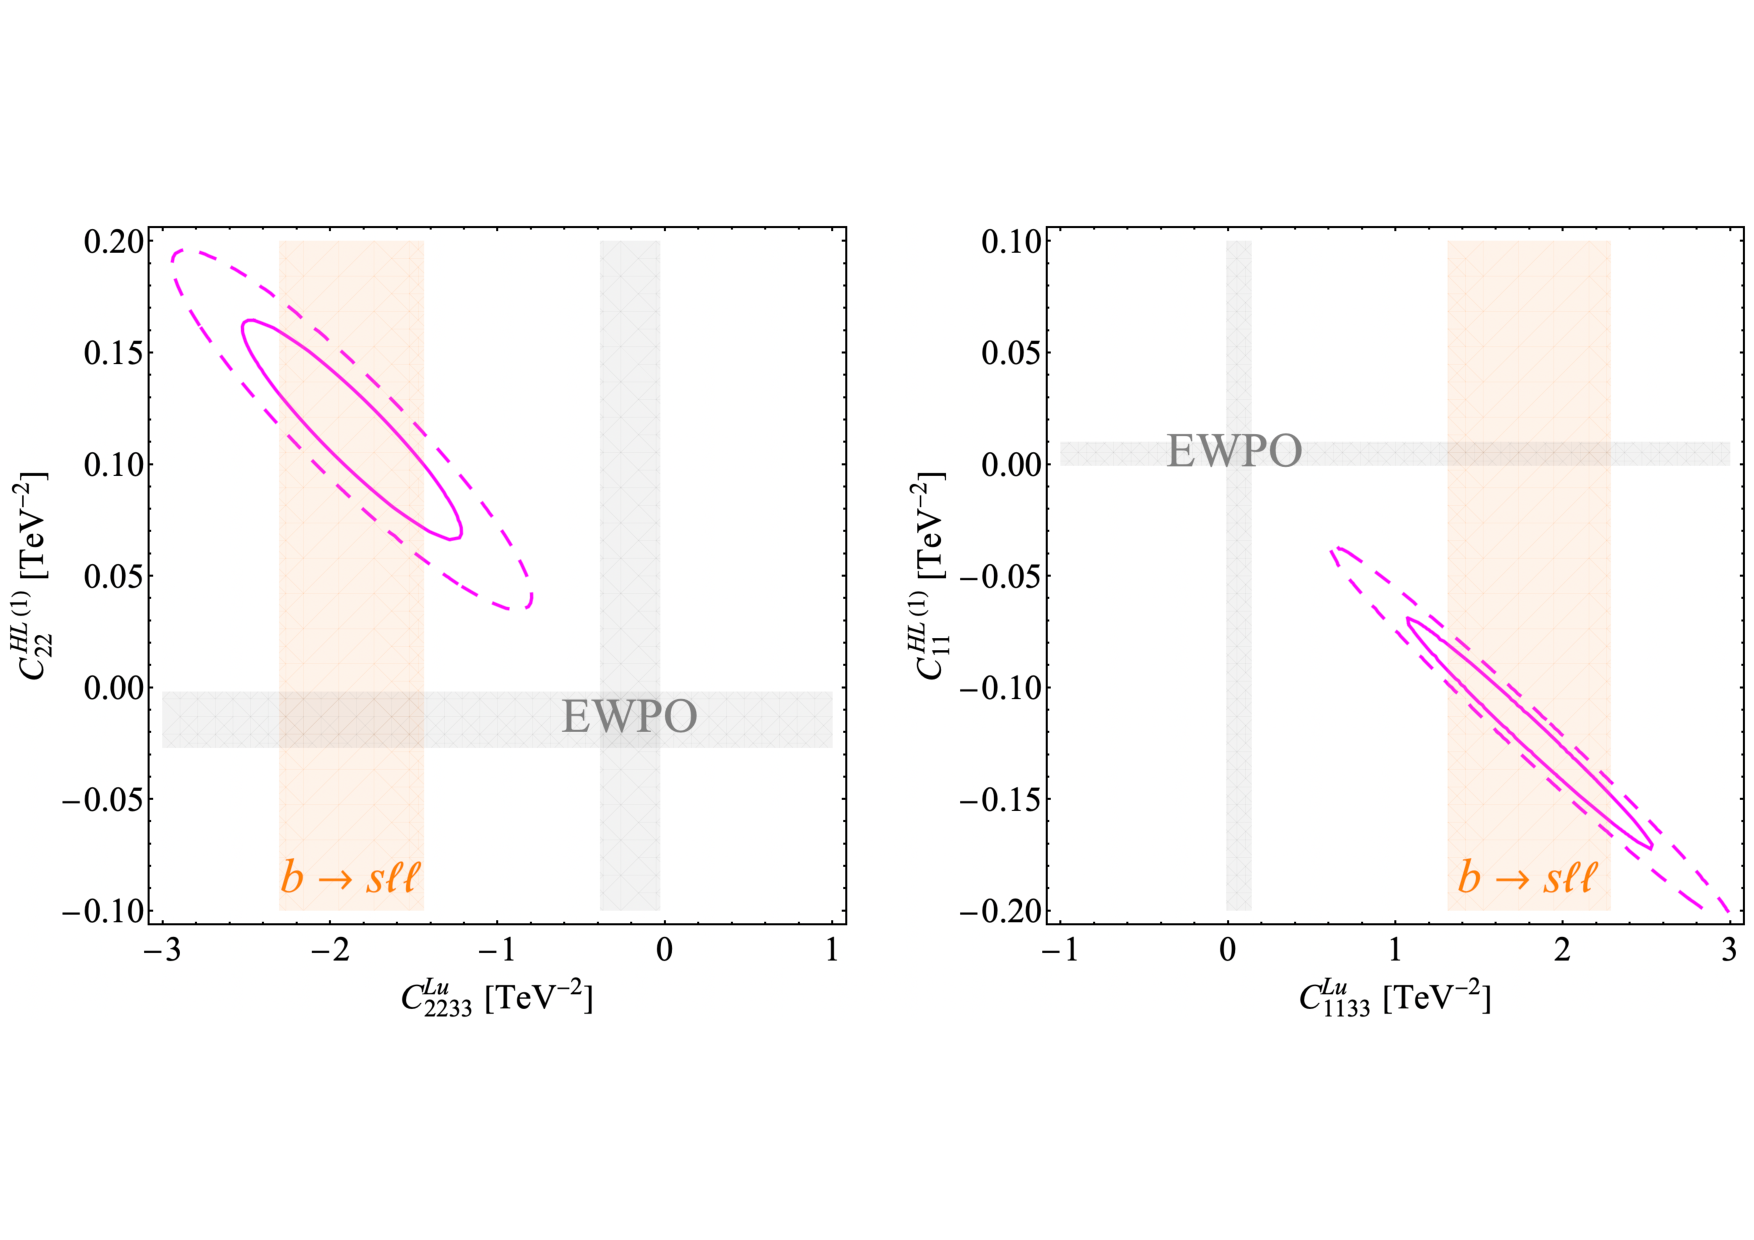
\includegraphics[width=\textwidth]{figures/CHL_CLu.pdf}
	\caption{ A minimal solution for the flavour anomalies within SMEFT, while respecting EWPO. The left panel shows the four-fermion operators involving the muon and on the right the electronic solution is shown. EWPO fits are the grey regions, while the $b \to s\ell \ell$ measurements fits with PDD ansatz are highlighted by the orange bands. The combined fit's 1 and 2$\sigma$ contours are magenta coloured.This plot has been published in~\cite{Alasfar:2020mne}.  } 
	\label{fig:2D_correlations}
\end{figure}

%Then, in \autoref{fig:2D_correlations} we show in orange the overall constraint from $b \to s \ell \ell$ data on $C^{Lu}_{\ell \ell 3 3}$ within the most conservative approach to long-distance effects, i.e. the PDD one. In particular, in the left (right) panel we report the constraint on the muonic (electronic) scenario. In the same figure, we highlight with the vertical gray band the bound derived from the full correlated set of EWPO on the same operator. From the comparison of the orange and gray single-operator bounds, the tension between flavour and EW measurements is manifest at the 3$\sigma$ level in the left panel of \autoref{fig:2D_correlations}. 
%
%Most importantly, in the same figure we display in (dashed) magenta the 1(2)$\sigma$ contour where EW data are reconciled with the one-loop MFV explanation of $B$ anomalies when a combined fit of the NP contributions from these two operators is performed. {Therefore, heavy BSM degrees of freedom that, once integrated out, generate sizeable contributions both  to the Wilson coefficient of $O^{HL^{(1)}}_{\ell \ell}$ and of $C^{Lu}_{\ell \ell33}$ are the key aspect of this scenario that addresses $B$ anomalies without requiring sources of flavour violation beyond SM ones.}
%It gets even more pronounced in the right panel due to the precise probe of NP that EW gauge-boson couplings to electrons provide. In the same \autoref{fig:2D_correlations}, we also show with the horizontal gray band the result of the EWPO constraints applied this time on the NP contribution coming exclusively from the operator $C^{HL^{(1)}}_{\ell \ell}$. Note that this operator would also contribute to $R_{K^{(*)}}$ at one loop, but the size needed would be $\mathcal{O}(1)$ and it is out of scale in the vertical axis of the plot.
Finally, note that the role played here by $\mathcal{O}_{Lu}^{\ell \ell 3 3}$ could be shared, in part, with $\mathcal{O}_{eu}^{\ell \ell 3 3}$, depending on how much departure is actually required from the fully left-handed solution to $B$ anomalies. As already noted, this fact critically depends on the information stemming from the angular analysis of $B \to K^{*} \mu \mu$~\cite{Ciuchini:2019usw}. On general grounds, to relieve the bounds from EWPO, the presence of $\mathcal{O}_{eu}^{\ell \ell 3 3}$ would also necessitate sizeable NP effects from $\mathcal{O}_{\phi e}^{\ell \ell}$, thus leaving us with a maximum of four needed operators to explain the flavour anomalies without being excluded by EWPO or including complex flavour structures.


%%%%%%%%%%%%%%%%%%
\section{Potential UV models}
\label{sec:UVtoymodels}
%%%%%%%%%%%%%%%%%%
%As a last comment of this section we would also like to highlight that in the class of models considered the prediction for the LUV observable $R_{K}$ is always close to the one for $R_{K^{*}}$: any hint of NP coming from $R_{K^{*}}/R_{K} \neq 1$~\cite{Hiller:2014ula,Hurth:2014vma,Hiller:2014yaa,Hiller:2017bzc} would not be addressed within the NP models considered here, mainly involving the operators in eq.~\eqref{eq:SMEFT_op_HL} and~\eqref{eq:SMEFT_op_loop_lu}. In the following sections we will put our focus on the economic EFT scenario captured in \autoref{fig:2D_correlations} to build up simple UV scenarios realizing the EFT picture here delineated.
In this section we discuss how the lesson derived from the SMEFT picture illustrated, in particular, in \autoref{fig:2D_correlations}, can be realized in a minimal extension of the SM. Here, we explicitly show how models involving a new $Z^\prime$ gauge boson around the TeV scale provide the most economic example of the correlations advertised in the previous section. 
This can be achieved if we have a $Z^\prime$ coupled both to top and lepton SM fields.
These couplings can be obtained introducing vector-like top and muon/electron partners reasonably close to the EW scale~\cite{Kamenik:2017tnu,Fox:2018ldq}, making this class of models potentially interesting also from the point of view of naturalness in the Higgs sector.
Finally, we will also briefly comment on possible alternative scenarios that can be obtained with leptoquarks.

%%%%%%%%%%%%%%%%%%
\subsection{\texorpdfstring{Z$^{\prime}$}{Z'} with vector-like partners}
\label{sec:mod_Zprime}
%%%%%%%%%%%%%%%%%%

Let us start with the baseline presented originally in ref.~\cite{Kamenik:2017tnu}. A simple extension of the SM, able to address $B$ anomalies, and  that does not introduce any explicit new source of flavour violation, can be conceived as follows:
\begin{itemize}
	\item The SM gauge group, $SU(3)_{c} \otimes SU(2)_{L} \otimes U(1)_{Y}$, is extended by a new Abelian gauge group, $U(1)_{X}$, under which SM fields are neutral;
	\item There is a new complex scalar field $\mathcal{S}$ that spontaneously breaks $U(1)_{X}$, giving a mass to the gauge boson $X_{\mu}$ equal to $m_{Z^{\prime}} = g_{X} \langle \mathcal{S} \rangle $;
	\item A coloured vector-like top partner, $\mathcal{T}$, properly charged under $U(1)_{X}$ and $U(1)_{Y}$ can mix with the right-handed top-quark field $u_{3}$ via a Yukawa interaction with $\mathcal{S}$; 
	\item A vector-like muonic partner, $\mathcal{M}$, doublet of $SU(2)_{L}$ and charged under $U(1)_{X,Y}$, can mix with the muonic doublet $L_2$ via another Yukawa coupling of $\mathcal{S}$;
	\item The couplings controlling the kinetic-mixing term, $X_{\mu \nu} B^{\mu \nu}$, and the quadratic scalar mixing, $\mathcal{S}^{\dagger}\mathcal{S} H^{\dagger} H$, are set to be phenomenologically negligible.\footnote{Using naive dimensional analysis, both kinetic and scalar quadratic mixing should appear beyond the tree level suppressed at least by a loop factor and the corresponding SM-partner rotation angles.} 
\end{itemize}

Then, the UV model is completely characterized by eight new parameters: the gauge coupling $g_{X}$, the mass $\mu_{\mathcal{S}}$ and quartic $\lambda_{\mathcal{S}}$ of the renormalizable potential of $\mathcal{S}$, the new Yukawa couplings $Y_{\mathcal{T},\mathcal{M}}$, here taken to be real, and the vector-like mass-term parameters $M_{\mathcal{T},\mathcal{M}}$.
In particular, the Lagrangian of the model contains the following terms:
\begin{equation}
	\label{eq:new_Yukawa_Mu}
	M_{\mathcal{T}} \bar{\mathcal{T}_R} \mathcal{T}_L + M_{\mathcal{M}} \bar{\mathcal{M}}_R \mathcal{M}_L +
	Y_{t} \bar{u}_{3} \tilde{H}^\dagger Q_{3}  
	+ Y_{\mathcal{T}} \bar{u}_{3} \mathcal{T}_L \mathcal{S} 
	+ Y_{\mu} \bar{e}_{2}  H^\dagger  L_{2}
	+ Y_{\mathcal{M}}\bar{\mathcal{M}}_R L_{2} \mathcal{S} + \mathrm{h.c.}  \ , 
\end{equation}
that characterize the mixing pattern of SM fields and vector-like partners.\footnote{Note that upon an opposite $U(1)_{X}$ charge assignment for the vector-like fermionic partners than the one implicitly assumed, one should replace in eq.~\eqref{eq:new_Yukawa_Mu} $\mathcal{S}$ with $S^{\dagger}$.}
Symmetry breaking of $U(1)_X$ is triggered by $\langle \mathcal{S} \rangle^2 = -\mu^2_{\mathcal{S}}/(2 \lambda_{\mathcal{S}}) \equiv \eta^2 \neq 0$, that implies the following fermionic mixing patterns:
\begin{eqnarray}
	\label{eq:Mixing_Partner}
	& \textrm{top sector:} & \ 
	\left(  \begin{array}{cc}
		\bar{u}_3 & \overline{\mathcal{T}}_R
	\end{array} \right) \, \begin{pmatrix}
		\frac{Y_t  \, v}{\sqrt{2}} \ &  \frac{Y_{\mathcal{T}} \eta}{\sqrt{2}} \ \\
		0 \ & \ M_\mathcal{T}
	\end{pmatrix} \,
	\left(  \begin{array}{c}
		U_3 \\  \mathcal{T}_L
	\end{array} \right) \ + \ \mathrm{h.c.} \, , \\
	& \textrm{muon sector:} & \ 
	\left(  \begin{array}{cc}
		\bar{e}_2 & \overline{\mathcal{M}}_{R}
	\end{array} \right) \, \begin{pmatrix}
		\frac{Y_\mu v}{\sqrt{2}} \ & 0\ \\
		\frac{Y_{\mathcal{M}} \eta }{ \sqrt{2}}  \ & \ M_\mathcal{M}
	\end{pmatrix} \,
	\left(  \begin{array}{c}
		E_{2} \\  \mathcal{M}_L
	\end{array} \right) \ + \ \mathrm{h.c.} \, , \nonumber
\end{eqnarray}
where $U_{i}$ ($E_{i}$) indicates the $Q_{i}$-component ($L_{i}$-component) with weak isospin $1/2$ (-1/2). Using the determinant and trace of the squared mass matrices, one can easily show that the eigenvalues $m_{t,\mathcal{T}}$ and $m_{\mu,\mathcal{M}}$ must satisfy~\cite{Kamenik:2017tnu}:
\begin{eqnarray}
	\label{eq:Mass_Eigenvalues}
	m_{t,\mu} \,  m_{\mathcal{T,M}} & = & \frac{1}{\sqrt{2}} Y_{t,\mu} v M_{\mathcal{T,M}} \ , \\ m_{t,\mu}^2 + m_{\mathcal{T,M}}^2 & = & 
	M_{\mathcal{T,M}}^2 + \frac{1}{2} (Y_{t,\mu} \, v)^2 + \frac{1}{2} (Y_{\mathcal{T,M}} \, \eta)^2 \ , \nonumber
\end{eqnarray}
that in the decoupling limit clearly yield: $m_{t,\mu} \simeq Y_{t,\mu} v / \sqrt{2}$, $m_{\mathcal{T,M}} \simeq M_{\mathcal{T,M}}$.

Defining for the top sector the rotation matrix from the interaction to the mass basis following the convention:

\begin{equation}
	\label{eq:rot_phys_states} 
	\left(  \begin{array}{c}
		t_{R (L)} \\  \mathcal{T}^{\prime}_{R (L)}
	\end{array} \right) = \,
	\begin{pmatrix}
		\cos \theta^{t}_{R(L)} \ & \ - \sin \theta^{t}_{R(L)} \ \\
		\sin \theta^{t}_{R(L)}  \ & \ \ \ \, \cos \theta^{t}_{R(L)}
	\end{pmatrix} \,
	\left(  \begin{array}{c}
		u_{3} (U_{3}) \\  
		\mathcal{T}_{R (L)}
	\end{array} \right) \ ,
\end{equation}
and doing similarly for the muonic sector, the mixing angles between SM fields, $t$ and $\mu$,  and their partner mass eigenstates, $\mathcal{T}^{\prime}$ and $\mathcal{M}^{\prime}$, can be conveniently expressed in terms of the dimensionless ratios $\xi_{\mathcal{T,M}}$ and $\varepsilon_{t,\mu}\, $:
\begin{eqnarray}
	\label{eq:partner_mixing}
	& \  \tan 2 \theta_{R}^{t} = \frac{2 \xi_{\mathcal{T}}}{\xi_{\mathcal{T}}^2-\varepsilon_{t}^2-1} \, , \, 
	\ \, \tan 2 \theta_{L}^{t} = \frac{2 \varepsilon_{t}}{\xi_{\mathcal{T}}^2-\varepsilon_{t}^2 +1} \, , \,   \textrm{with} \ \varepsilon_{t} \equiv \frac{Y_{t} v}{Y_{\mathcal{T}} \eta},~\xi_{\mathcal{T}} \equiv \frac{\sqrt{2} M_{\mathcal{T}}}{\eta Y_{\mathcal{T}}} \, ; \ \\
	& \  \tan 2 \theta_{R}^{\mu} = \frac{2 \varepsilon_{\mu}}{\xi_{\mathcal{M}}^2-\varepsilon_{\mu}^2+1} \, , \, 
	\tan 2 \theta_{L}^{\mu} = \frac{2 \xi_{\mathcal{M}}}
	{\xi_{\mathcal{M}}^2-\varepsilon_{\mu}^2 -1}  \, , \, 
	\textrm{with} \ \varepsilon_{\mu} \equiv \frac{Y_{\mu} v}{Y_{\mathcal{M}} \eta},~\xi_{\mathcal{M}} \equiv \frac{\sqrt{2} M_{\mathcal{M}}}{\eta Y_{\mathcal{M}}} \, .
	\nonumber
\end{eqnarray}
In a perturbative expansion in $\varepsilon_{t,\mu}$, eq.~\eqref{eq:partner_mixing} clearly shows that the mixing in the top sector proceeds mainly through $\tan\theta^{t}_{R} \simeq 1/\xi_{\mathcal{T}}$, while in the muonic sector one has  $\tan\theta^{\mu}_{L} \simeq 1/\xi_{\mathcal{M}}$ and very tiny $\tan\theta^{\mu}_{R}$.

Hence, for $\varepsilon_{t,\mu}/\xi_{\mathcal{T,M}}= Y_{t,\mu} v/\sqrt{2} M_{\mathcal{T,M}} < 1$, the leading couplings of the $Z^{\prime}$ boson to the SM fields correspond to right-handed tops and to left-handed muons as well as neutrinos according to:\footnote{In what follows, for $\eta \sim \mathcal{O}(v)$ we will have $\xi_{T} \sim \mathcal{O}(1)$; consequently, $\varepsilon_{t} \sim \mathcal{O}(v/M_{\mathcal{T}})$.}
\begin{eqnarray}
	\label{eq:Zprime_to_SM}
	g_{Z^{\prime} t_{R}} & = & g_{X} \sin^2 \theta_{R}^{t} = \frac{g_{X}}{ 1+ \xi^2_{\mathcal{T}}} + \mathcal{O}\left( \varepsilon_{t}^2/\xi_{\mathcal{T}}^2 \right) \, , \\
	g_{Z^{\prime} \mu_{L} (\nu)} & = &  g_{X} \sin^2 \theta_{L}^{\mu} = \frac{g_{X}}{1 + \xi^2_{\mathcal{M}}} 
	+ \mathcal{O}\left( \varepsilon_{\mu}^2 /\xi_{\mathcal{M}}^2 \right) \, ,
\end{eqnarray}
with $g_{Z^{\prime} t_{L} (\mu_{R})}$ being non-negligible only at order $\varepsilon_{t  (\mu)}^2/\xi_{\mathcal{T(M)}}^2$.
Consequently, integrating out the $Z^{\prime}$ relevantly generates the operator $O^{L u}_{2233}$ with Wilson coefficient:
\begin{equation}
	\label{eq:CLu_Zprime}
	C^{L u}_{2233} = - \frac{g_{Z^{\prime} t_{R} } g_{Z^{\prime} \mu_{L}} }{m_{Z^{\prime}}^2} \simeq - \frac{1}{(1+ \xi^2_{\mathcal{T}})(1+ \xi^2_{\mathcal{M}}) \, \eta^{2}} \ ,
\end{equation}
%
together with four-fermion operators built of $t_{R}$ or $\mu_{L},\nu$  fields that can be potentially probed at collider and by experimental signatures like $\nu$-trident production. 

From eq.~\eqref{eq:CLu_Zprime} it is clear that in order to have $|C^{L u}_{2233}| \sim 2 $ TeV$^{-2}$ as highlighted in \autoref{fig:2D_correlations}, one needs to rely on a relatively low symmetry-breaking scale $\eta \lesssim$~TeV;\footnote{Note that even for masses as low as $\mu_{\mathcal{S}} \sim \mathcal{O}(v)$, for $\eta \simeq v$ and $\lambda_{\mathcal{S}} \sim \mathcal{O}(1)$, the interactions of $\mathcal{S}$ do not alter the phenomenology discussed here since the largest $\mathcal{S}$-generated effects are still suppressed as $\mathcal{O}(\varepsilon_{t}^2/\xi^2_{\mathcal{T}})$.} for $m_{Z^{\prime}} \sim$~TeV this implies $g_{X} \gtrsim$~1. In \autoref{fig:Zp_constraints} we show the $1\sigma$ region corresponding to the explanation of $B$ anomalies via eq.~\eqref{eq:CLu_Zprime} in the parameter space $\xi_{\mathcal{T,M}}$, fixing the gauge coupling $g_{X} = m_{Z^{\prime}}/\eta$ for a tentative $Z^{\prime}$ gauge boson at the~TeV scale and the VEV of the new scalar field $\mathcal{S}$ set to $\eta = 250$~GeV and $\eta = 500$~GeV  in the left and right panel, respectively. In the same plot, we re-interpret in our scenario the most relevant collider constraints originally identified in ref.~\cite{Camargo-Molina:2018cwu}. 

\begin{figure}[htpb!]
	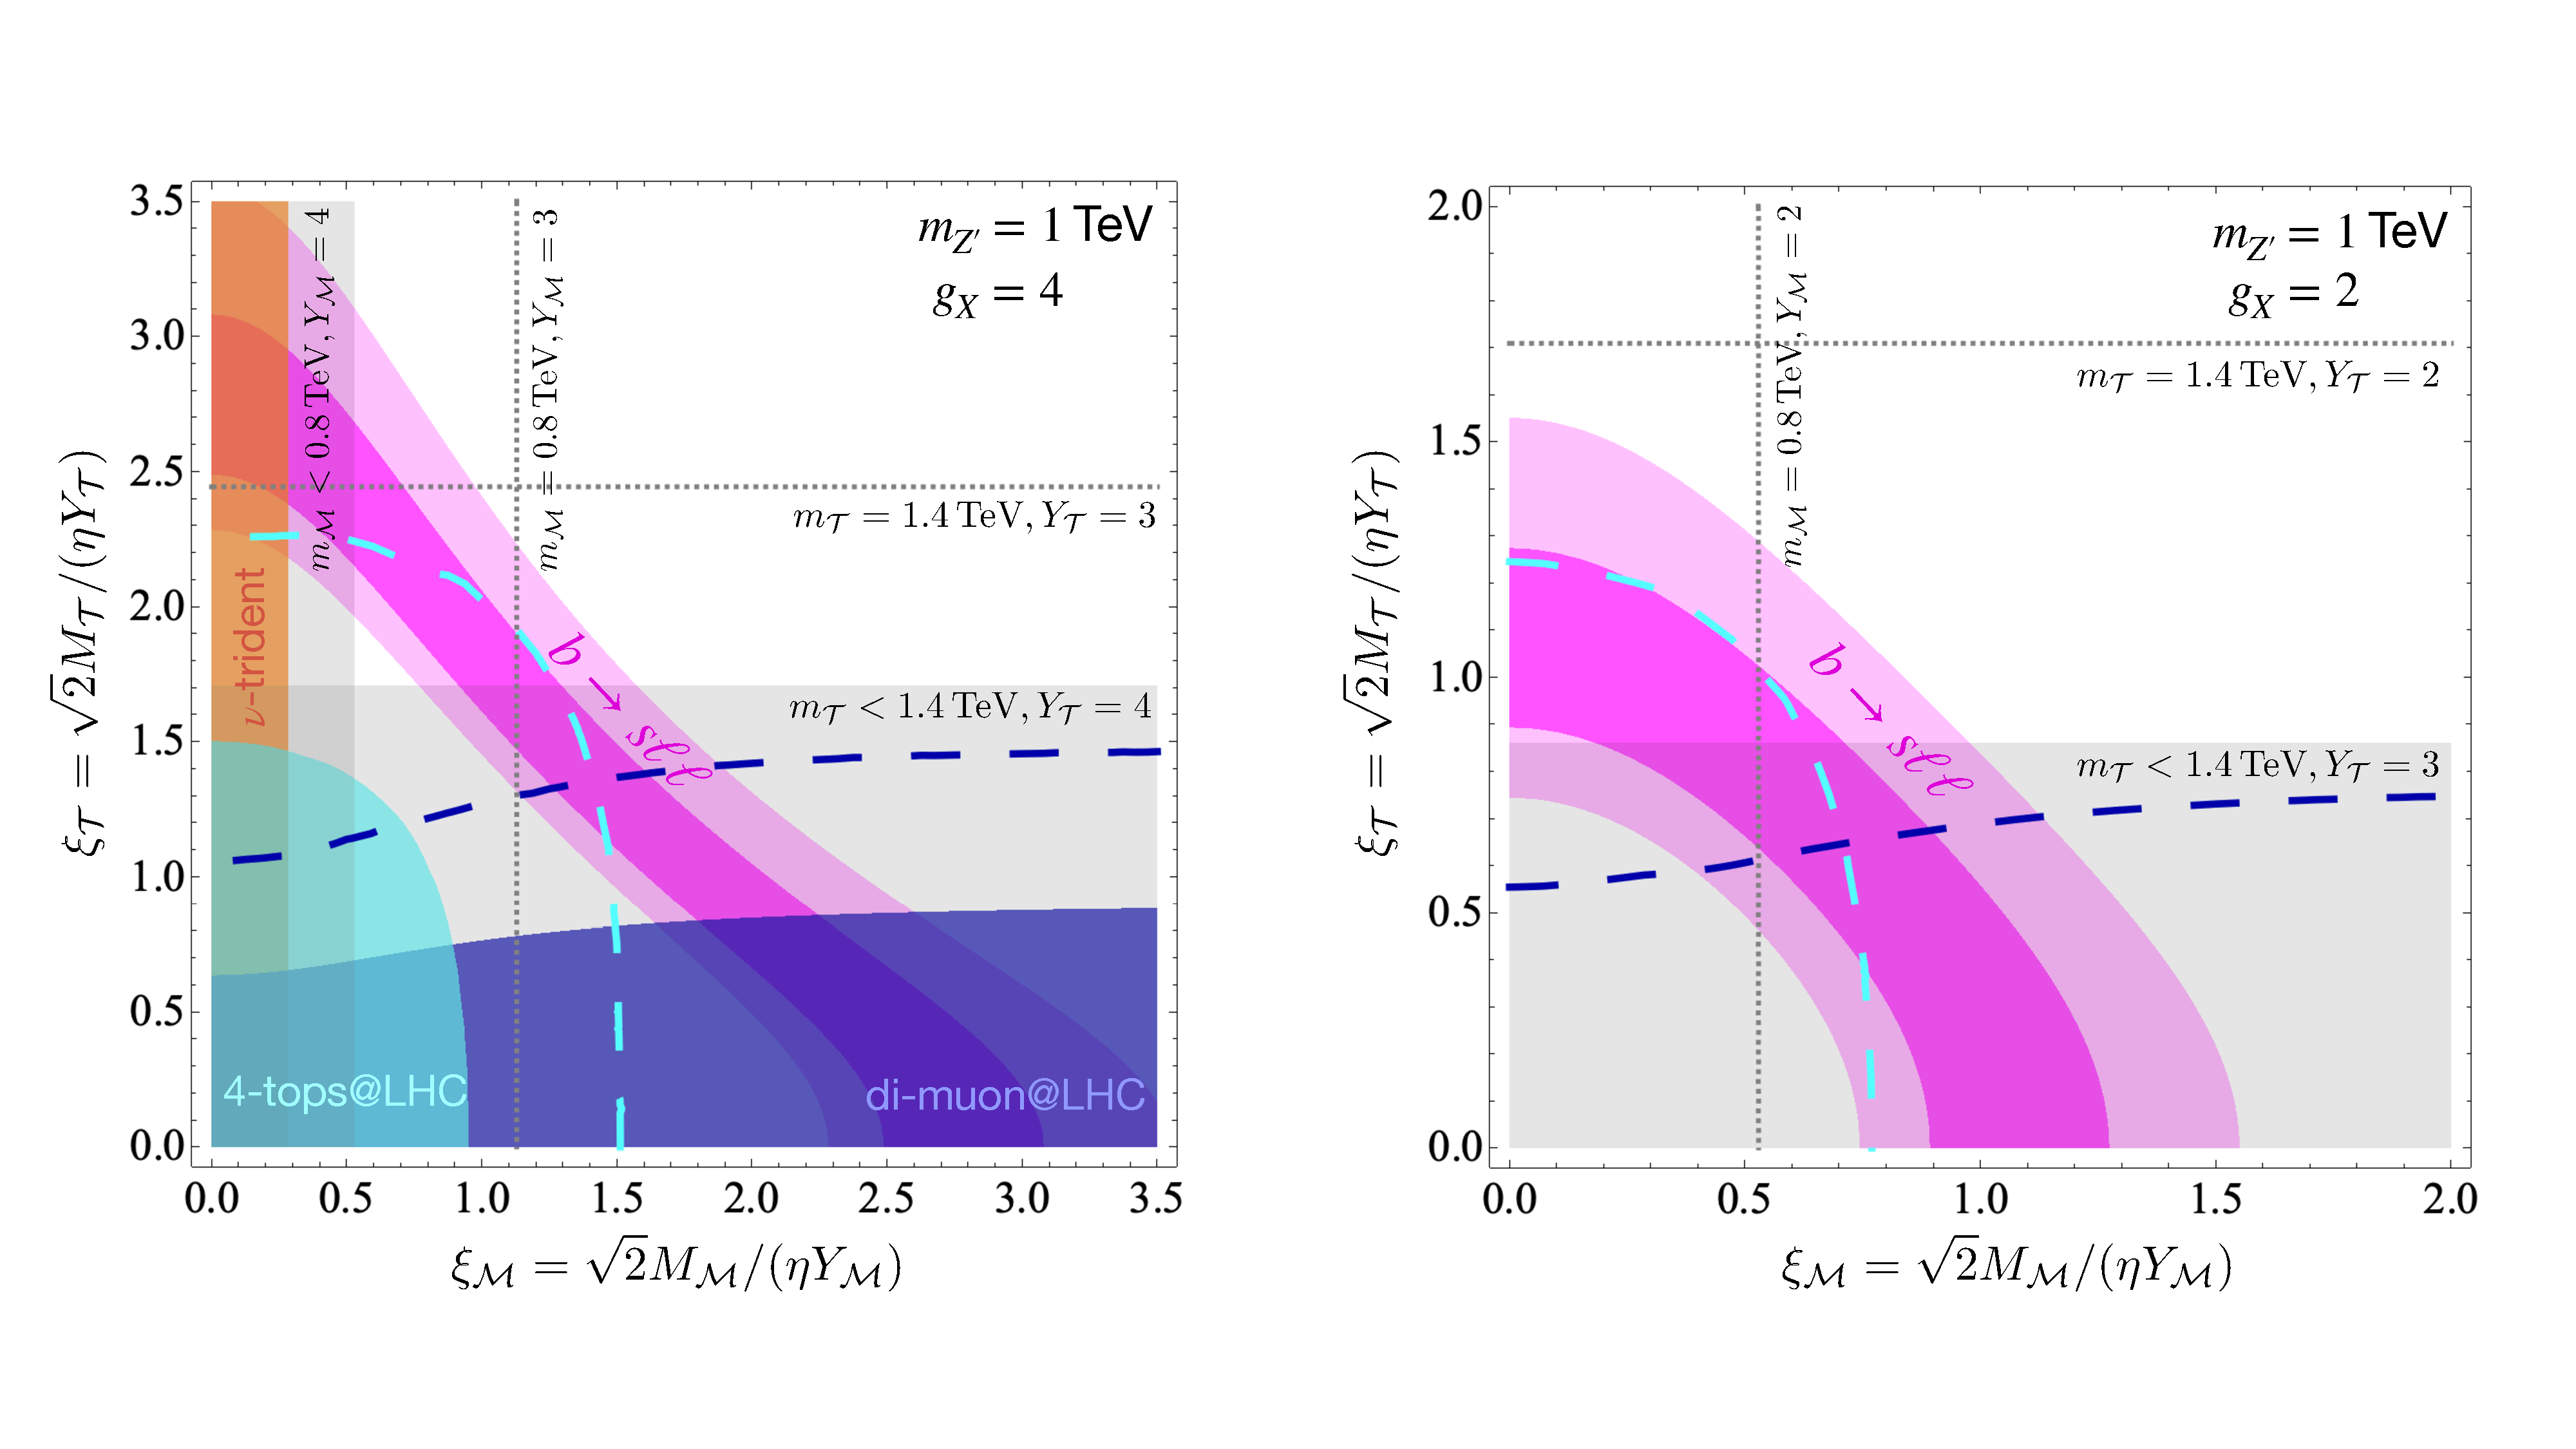
\includegraphics[scale=0.235]{figures/Zprime_constraint_CLu.pdf}
	\caption{\it 68\% (95\%) probability region in (lighter) magenta for the minimal $Z^{\prime}$ model that addresses $B$ anomalies in the parameter space identified by eq.~\eqref{eq:CLu_Zprime}, with $\eta = m_{Z^{\prime}}/4$ (left panel), and $\eta =  m_{Z^{\prime}}/2$ (right panel), for $m_{Z^{\prime}} = 1~\textrm{TeV}$. Relevant LHC constraints are reported in blue and cyan regions according to the analysis originally performed in ref.~\cite{Camargo-Molina:2018cwu}, together with the corresponding collider projections at 300~fb$^{-1}$. Finally, the gray regions underlie the parameter space where the mass of the vector-like partner lies below current collider limits for a fixed Yukawa coupling as explicitly reported, while dashed lines show the corresponding shift of the limit due to a smaller value of the same type of Yukawa coupling.}    
	\label{fig:Zp_constraints}
\end{figure}

For small values of $\xi_{\mathcal{M}}$, the measurement of neutrino-trident production performed in~\cite{Mishra:1991bv} is effective, and its constraint is reported at the 2$\sigma$ level with the orange vertical band.
Under the reasonable assumption that the $Z^{\prime}$ boson is mainly produced at tree level in association with the $ t \bar{t}$ pair, in the blue region we show the 95\% high-$p_{T}$ constraint stemming from the recasting of the $p p \to \mu^{-} \mu^{+} t \bar{t}  $ search at ATLAS~\cite{Aaboud:2017buh}, while in cyan we report the expected constraint on the model from the 4-tops analysis of CMS~\cite{Sirunyan:2017roi}, see ref.~\cite{Camargo-Molina:2018cwu} for further details. From the same work, we also adopt the expected collider constraints for future projected luminosity corresponding to 300~fb$^{-1}$, shown with dashed lines.  Note that these projections become of fundamental importance when it comes to probe the interesting 1$\sigma$ region connected to $B$ anomalies. 
In particular, the right panel in \autoref{fig:Zp_constraints} captures the benchmark for a promising discovery at the High-Luminosity LHC.

Finally, in the same figure, fixing the partner Yukawa coupling to  $\mathcal{O}(1)$ values as reported in the two panels, we mark in gray the region corresponding to the bound on the mass of the vector-like partner expected from collider, taken to be $m_{\mathcal{T}} = 1.4$~TeV from the search at ATLAS in ref.~\cite{Aaboud:2018uek}, and $m_{\mathcal{M}} = 0.8$~TeV from the CMS analysis of ref.~\cite{Sirunyan:2019ofn}.

As already discussed, the scenario depicted in \autoref{fig:Zp_constraints} remains viable under the lens of EW precision as long as we also have some heavy new dynamics yielding at the EW scale an imprint of $O^{HL^{(1)}}_{22}$ consistently with the correlation obtained in the left panel of \autoref{fig:2D_correlations}. 

A simple way to obtain such NP contribution would be to consider the joint effect that the leptonic mixing of the vector-like partner would have together with the kinetic mixing of the $Z^{\prime}$, so far neglected. The $Z$-$Z^{\prime}$ mixing could also originate from charging the new scalar field $\mathcal{S}$ under both Abelian gauge groups, introducing a small misalignment with the standard hypercharge $U(1)_{Y}$ in the UV. However, the required mixing of the $Z^{\prime}$ would end up mediating light-quark pair annihilation into muons: the typical size of the Wilson coefficient of this four-fermion operator would be $\mathcal{O}(g_{Y}^2/m^2_{Z^{\prime}})$, in net tension with the di-muon bound from ATLAS~\cite{Aaboud:2017buh}, probing NP scales as high as $20$~-~$40$~TeV for $\mathcal{O}(1)$ (dimensionless) couplings. Hence, we rule out here this possibility.

Interestingly, it is still possible to generate $O^{HL^{(1)}}_{22}$ without relying on the $Z$-$Z^{\prime}$ mixing, but rather invoking the presence in the UV theory of additional new vector-like leptonic states~\cite{Thomas:1998wy,delAguila:2008pw}. These ones may be phenomenologically interesting in relation  to the problem of the origin of neutrino masses as well as for the prediction of the anomalous magnetic moment $(g-2)_{\mu}$~\cite{Kannike:2011ng}, and may give peculiar multi-lepton signatures at colliders~\cite{Kumar:2015tna,Bhattiprolu:2019vdu}.

In the most economic scenario, we may consider the presence in the UV theory of a pair of new vector-like muonic partners: a singlet of $SU(2)_{L}$, $S_{Y}$, and a triplet of $SU(2)_{L}$, $T_{Y}$, 
where in both cases the subscript $Y$ denotes the hypercharge of the fermion.
%of hypercharge $Y$. 
These fields would have their own mass terms controlled by the parameters $M_{S_{Y},T_{Y}}$, and interact with the SM doublet $L_{2}$ via the Yukawa couplings $\mathcal{Y}_{S_{Y},T_{Y}}$ according to:
\begin{equation}
	\label{eq:Yuk_singl_tripl}
	\mathcal{Y}_{S_{0}} \bar{S}_{0,R} \tilde{H}^{\dagger} L_{2} + \mathcal{Y}_{T_{0}} \bar{T}^{A}_{0,R} \tau^{A} \tilde{H}^{\dagger} L_{2} + \textrm{h.c.}  \ ,
\end{equation} 
where we have reported the case of vector-like muonic partners with hypercharge $Y=0$. We assume the new Yukawa couplings to be real. Another possibility of interest may be the one of replacing in eq.~\eqref{eq:Yuk_singl_tripl} $\tilde{H} = i \tau^{2} H^*$
with the Higgs doublet, $H$, and involve then the pair of vector-like partners with hypercharge $Y=1$. 

Integrating out these vector-like states from the theory would generate contributions related to $\mathcal{O}^{HL^{(1,3)}}$ ~\cite{delAguila:2008pw,Kannike:2011ng} of the form:
\begin{eqnarray} 
	\label{eq:matching_CHL}
	C^{HL^{(1)}}_{22 } & = &
	\ \ \frac{ \mathcal{Y}^{2}_{S_{0}}}{4 M_{S_{0}}^2} 
	- \frac{ \mathcal{Y}^{2}_{S_{1}}}{4 M_{S_{1}}^2}
	+ \frac{ 3 \mathcal{Y}^{2}_{T_{0}}}{4 M_{T_{0}}^2}
	- \frac{ 3 \mathcal{Y}^{2}_{T_{1}}}{4 M_{T_{1}}^2} \ , \\
	C^{HL^{(3)}}_{22} & = & 
	- \frac{ \mathcal{Y}^{2}_{S_{0}}}{4 M_{S_{0}}^2}
	- \frac{ \mathcal{Y}^{2}_{S_{1}}}{4 M_{S_{1}}^2}
	+ \frac{ \mathcal{Y}^{2}_{T_{0}}}{4 M_{T_{0}}^2}
	+ \frac{ \mathcal{Y}^{2}_{T_{1}}}{4 M_{T_{1}}^2} \ . \nonumber
\end{eqnarray}
Clearly, in order to have $C^{HL^{(1)}}_{22} \sim 0.1$ and negligible $C^{HL^{(3)}}_{22}$\footnote{We have indeed verified that a scenario involving at the same time $C^{Lu}$ and $C^{HL^{(1,3)}}$ would not alter what already highlighted in~\autoref{fig:2D_correlations}, with the best-fit value for $|C^{HL^{(3)}}|$ turning out to be of $\mathcal{O}(10^{-2})$.}, 
one would need to rely on a tuning of the $Y=0$ triplet Wilson coefficient with one of the contributions coming from the singlet vector-like muonic partner. However, once generated at the NP scale $\Lambda \sim \mathcal{O}(M_{T_{0}}) \gg v$, we observe that the relation established between the triplet and singlet contributions to $O^{HL^{(1,3)}}$ would be stable under the RG flow of the SMEFT.

A final comment is needed for the electron scenario reported in the right panel of~\autoref{fig:2D_correlations}, that involves opposite signs for the Wilson coefficients of $O^{Lu}$ and $O^{HL^{(1)}}$ discussed so far. For the former, we note that the sign highlighted in the matching in eq.~\eqref{eq:CLu_Zprime} follows from having assumed the same sign for the charge of the vector-like top and muon partners under $U(1)_{X}$.
Hence, assuming the vector-like electron partner to have the opposite  $U(1)_{X}$ charge of the top-partner one would be sufficient to  accomplish $C^{Lu}_{1133} > 0$. (Of course, this would also imply a distinct use in eq.~\eqref{eq:new_Yukawa_Mu} of $\mathcal{S}$ and $\mathcal{S}^{\dagger}$ couplings in the Yukawa terms of the vector-like partners involved to keep the theory invariant under $U(1)_{X}$.) For what concerns the generation of $C^{HL^{(1)}}_{11} < 0 $, according to eq.~\eqref{eq:matching_CHL} one needs to correlate once again the contribution stemming from $S_{0}$, or from $S_{1}$, with the effect coming from a $SU(2)_{L}$ triplet, that now needs to be identified with $T_{1}$, namely the triplet of hypercharge $Y=1$.

Eventually, we wish also to comment on the possible role of the $O^{eu}$ operator, so far neglected in this discussion, but of potential relevance more in general. In fact, as mentioned earlier, the presence of $O^{eu}$ would be particularly needed in the case where hadronic corrections entering in the amplitude of $B \to K^* \ell \ell $ would be of the size originally estimated in~\cite{Khodjamirian:2010vf}. 
In that case, a solution to flavour anomalies would be preferred in the muonic channel with NP Wilson coefficient $C^{eu}_{2233}$ also substantially deviating from 0, as already discussed in \autoref{sec:GEN_EFT_results}. Then, one would need to involve also the operator $C^{He}_{22}$ to relieve possible tensions with EW precision. In a general picture, the required NP effects from $O^{He}_{11,22}$ can be obtained integrating out heavy vector-like $SU(2)_{L}$ leptonic doublets.


%%%%%%%%%%%%%%%%%%
\subsection{Leptoquark scenarios}
\label{sec:mod_Leptoquarks}
%%%%%%%%%%%%%%%%%%
An alternative way to reproduce the minimal EFT scenario of \autoref{fig:2D_correlations} would be via \emph{leptoquarks}~(LQ), particles generically predicted in grand unified  theories~(GUTs)~\cite{Pati:1974yy,PhysRevLett.32.438}.
Notoriously, LQ-induced dimension-six operators could be potentially dangerous as they would lead to proton decay at tree level, forcing to push their scale up to the GUT scale. However, the outcome may drastically change in models where the couplings of the LQs would be non-universal with respect to lepton and/or quark flavours. In such a case their mass could be much lower than what typically expected in GUTs and their signatures may actually be probed at present colliders. Interestingly, such LQs are candidates that could explain the lepton flavour universality violation -- even at the loop level here considered~\cite{Camargo-Molina:2018cwu,Coy:2019rfr} -- hinted in the recent LHCb and Belle data. However, this would imply generically a rather non-trivial flavour structure in the theory~\cite{Becirevic:2017jtw}. For a comprehensive survey of LQ models, see for instance~\cite{Buchmuller:1986zs,delAguila:2010mx,Alonso:2015sja,Dorsner:2016wpm,deBlas:2017xtg}. 

Here, we limit ourselves to the case of toy models that specifically generate the operators of interest, namely $C^{Lu}_{\ell \ell33}$ and $C^{eu}_{\ell \ell33} $, for $ \ell=1$ (electron)  or $ \ell=2$ (muon). In these peculiar LQ models we then assume that couplings between right-handed top quarks and light leptons are the only ones that actually matter for TeV phenomenology. 

In~\autoref{tab:LQmodels} we list the vector and scalar LQs that constitute the potential LQ candidates able to generate the solutions for $b \to s \ell \ell$ anomalies at one loop under scrutiny.  

\begin{table}[!ht]
	\centering
	{
		\begin{tabular}{ccc }
			\toprule
			Vector LQ: $\mathcal{V^\mu}$ & $SU(3)_{c} \otimes SU(2)_{L} \otimes U(1)_{Y}$ & Comments \\
			\midrule
			$ \bar L_\ell  \gamma_\mu (\tau^A) Q_3 \, \mathcal{V}^{\mu (A)} $ & $(\overline{\irrep{3}},\irrep{1}\,\text{or}\,\irrep{3}, -2/3 )$ & not of interest \\
			$  ( \mathcal{V^\mu} )^{\dagger} \,\bar e_\ell^c  \gamma_\mu Q_3 $ & $(\overline{\irrep{3}},\irrep{2}\,, 5/6 )$ & not of interest \\
			$\bar{L}^c_\ell \gamma_\mu u_3\, i\tau^2 \, \mathcal{V^\mu}$ & $(\overline{\irrep{3}},\irrep{2}, -1/6 )$ & generates $C^{Lu}_{\ell \ell 33} > 0$\\
			$ \overline {e}_\ell \gamma_\mu u_3\, \mathcal{V^\mu}$ & $(\overline{\irrep{3}},\irrep{1}, -5/3 )$ & generates $C^{eu}_{\ell \ell 33} < 0$ \\    
			\midrule
			Scalar LQ: $\mathcal{S}$ &  &  \\
			\midrule
			$\bar L_\ell (\tau^A) (i \tau^{2}) \, Q_3^{c} \,\mathcal{S}^{\dagger (A)} $ & $(\overline{\irrep{3}},\irrep{1}\,\text{or}\,\irrep{3} ,1/3 )$ & not of interest  \\    
			$\bar e_\ell Q_3 \,  i \tau^2 \mathcal{S} $ & $(\overline{\irrep{3}},\irrep{2} ,-7/6 )$ & not of interest \\
			$\bar L_\ell u_3\, \mathcal{S} $  & $(\overline{\irrep{3}},\irrep{2} ,-7/6 )$  & generates $C^{Lu}_{\ell \ell 33} < 0$ \\
			$\bar e_\ell^c u_3\, \mathcal{S}$ & $(\overline{\irrep{3}},\irrep{1} ,1/3 )$ & generates $C^{eu}_{\ell \ell 33} > 0$ \\
			\bottomrule
		\end{tabular}
	}
	\caption{Scalar and vector LQ interactions under scrutiny: LQs of interest for our analysis have to generate the dimension-six operators $O^{Lu,eu}_{\ell \ell 33}$.}
	\label{tab:LQmodels}
\end{table}

Looking back at \autoref{fig:2D_correlations}, from the table above we recognize as the most economic LQ scenario for the resolution of $B$ anomalies at one loop, the case of the vector LQ $ \mathcal V^\mu\sim(\overline{\irrep{3}},\irrep{2}, -1/6 )$ for LUV effects originating from electron couplings, and the scalar $\mathcal S\sim (\overline{\irrep{3}},\irrep{2} ,-7/6 )$ for the ones associated to muons.
The interaction terms of interest are:
\begin{equation}
	\mathcal{L}_{\mathcal V \bar f f} =  \tilde \lambda_{t e}  \, \bar L^c_1\gamma_\mu u_{3} \, i \tau^2 \mathcal V^\mu  + \mathrm{h.c.} 
	\ \ , \ \
	\mathcal{L}_{\mathcal S \bar f f} =  \lambda_{t \mu} \,  \bar L_2 u_{3} \mathcal{S}  + \mathrm{h.c.} ,
\end{equation}
leading to the corresponding matching condition:
\begin{equation}
	C^{Lu}_{1133} = +\frac{| \tilde \lambda_{t e}|^2}{M_{\mathcal V} ^2 }  
	\ \ , \ \ C^{Lu}_{2233} = -\frac{|  \lambda_{t \mu}|^2}{2 M_{\mathcal S}^2 } \ .
\end{equation}
In \autoref{fig:LQ_constraints} we report in (lighter) magenta the underlying 1(2)$\sigma$ region where $B$ anomalies are addressed in concordance with the minimal EFT picture of \autoref{fig:2D_correlations}. In the same plot, we also show a conservative estimate of the present LHC constraint on the mass of the LQ states considered, based on the dedicated collider study of ref.~\cite{Angelescu:2018tyl}.

\begin{figure}[htpb!]
	\centering 
	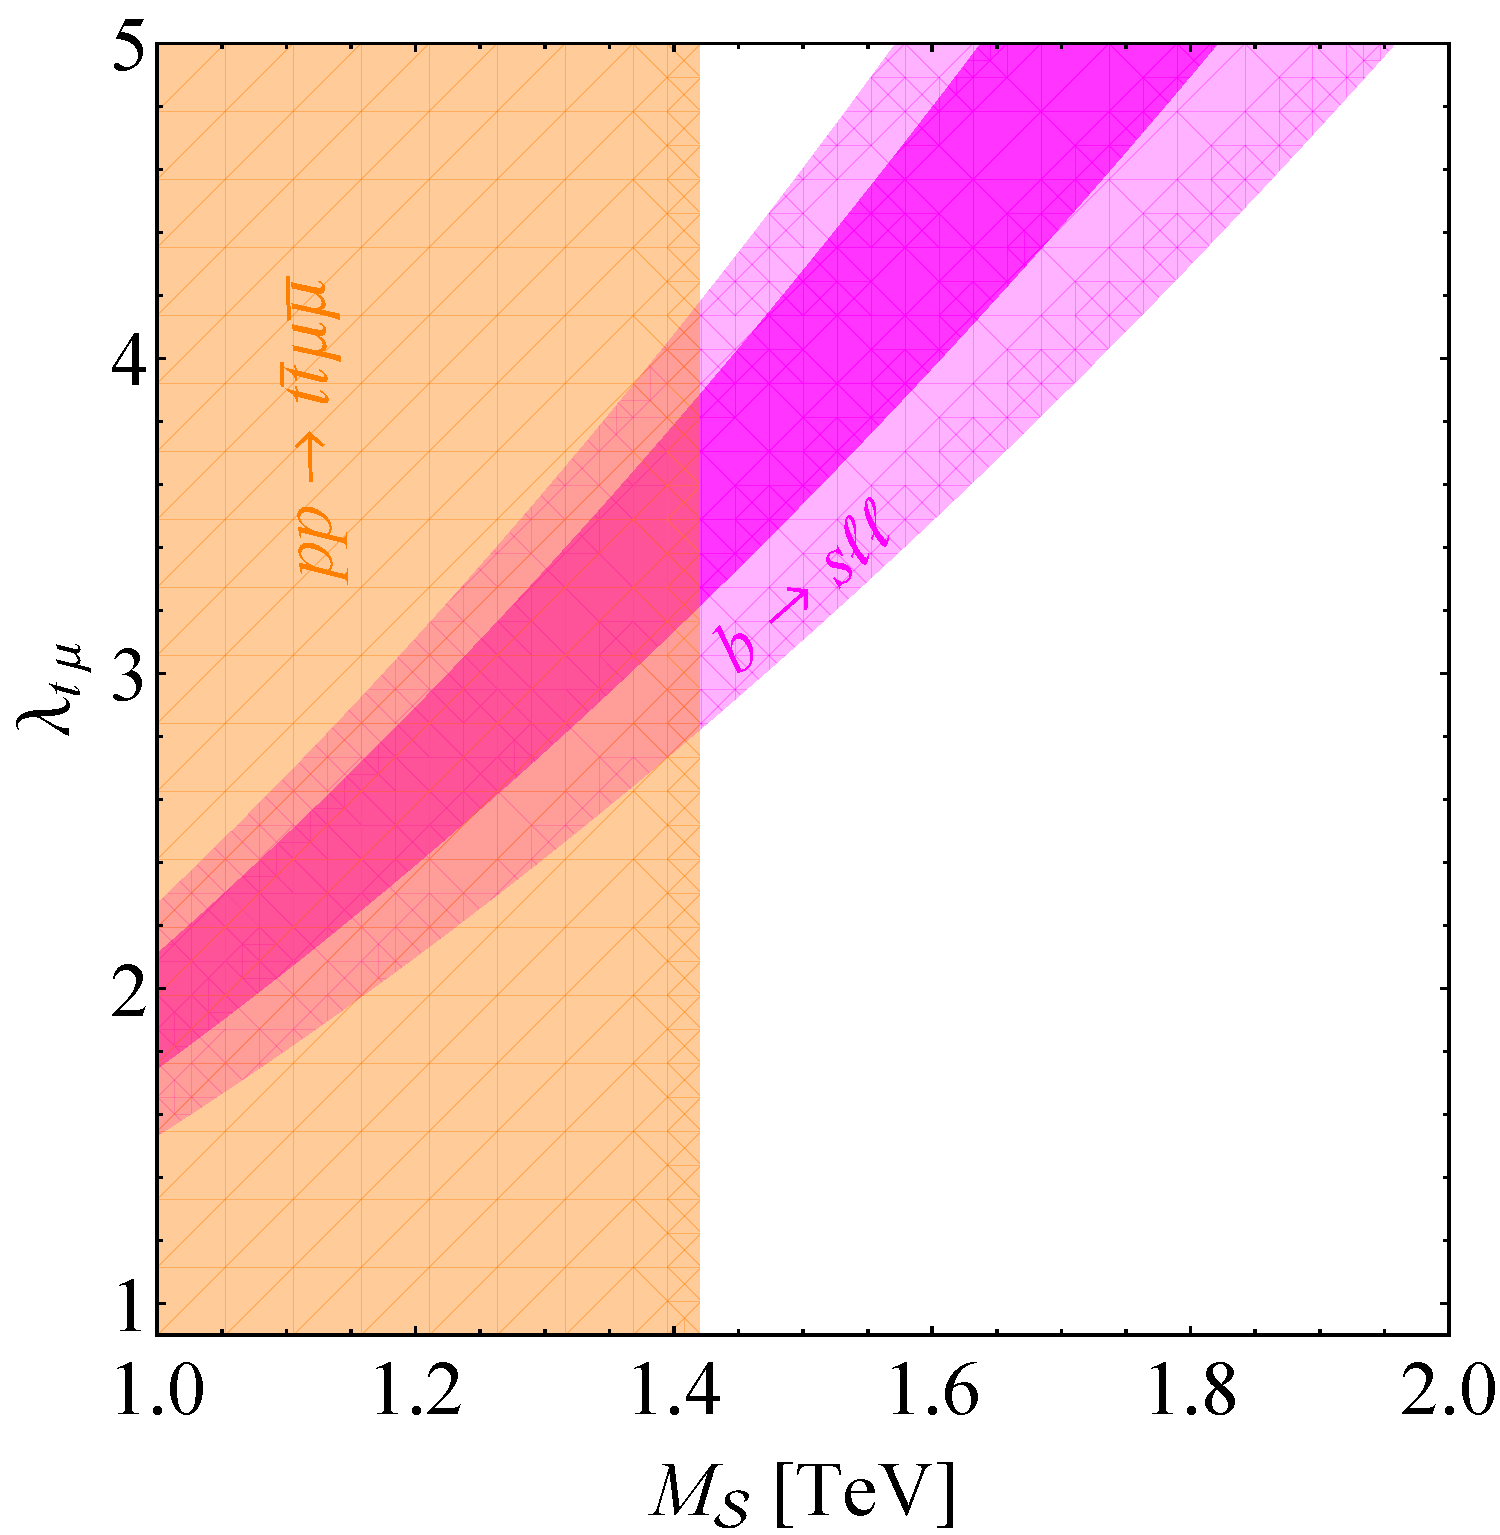
\includegraphics[width=0.45\linewidth]{figures/Scalar_LQ.pdf}
	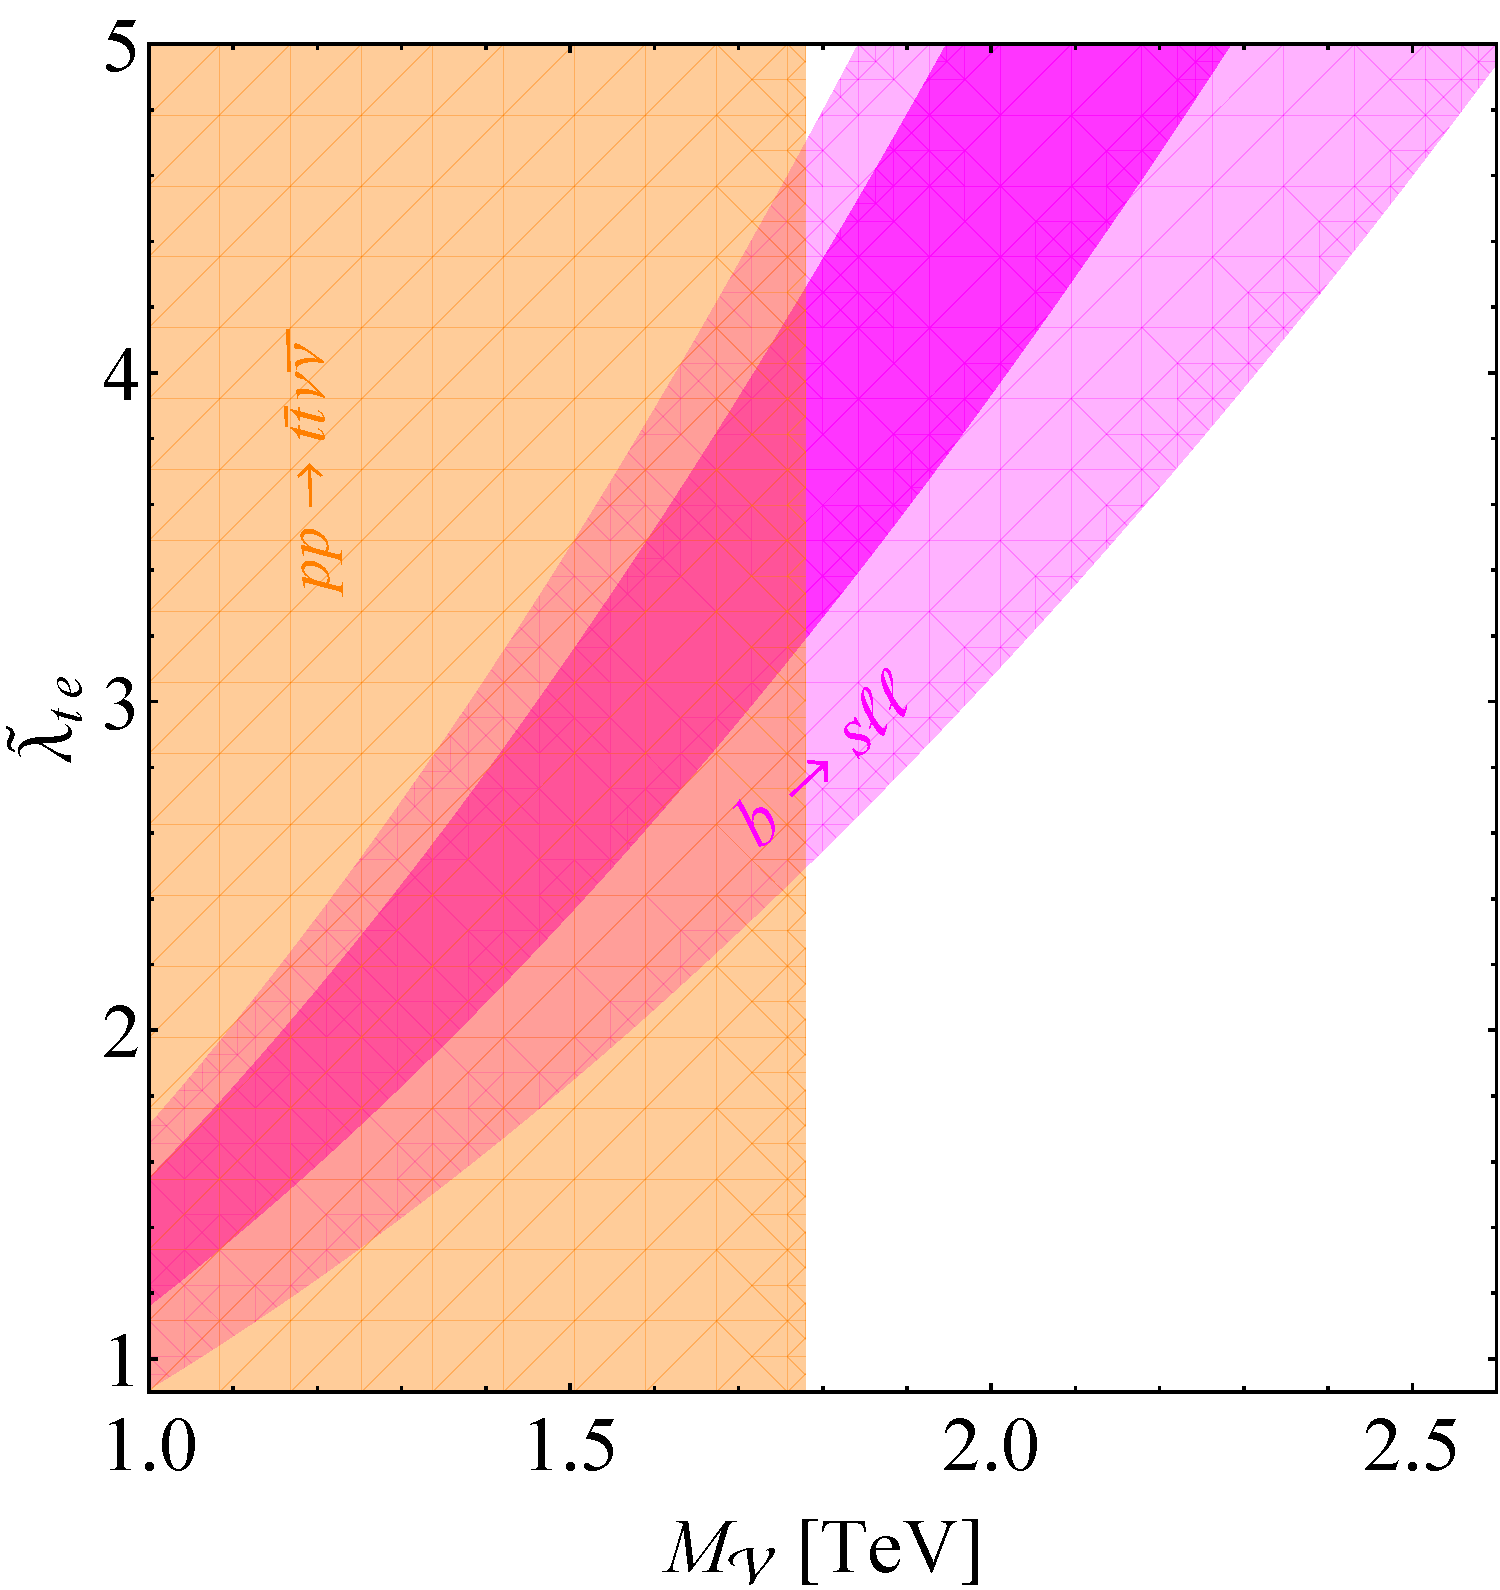
\includegraphics[width=0.435\linewidth]{figures/Vector_LQ.pdf}
	\caption{68\% (95\%) probability region in magenta for the LQ candidates addressing $b \to s \ell \ell$ anomalies at one loop. The scalar (vector) LQ corresponds to a solution with LUV effects related to muon (electron) couplings. A conservative bound on the corresponding LQ mass is reported according to the analysis of ref.~\cite{Angelescu:2018tyl}.}    
	\label{fig:LQ_constraints}
\end{figure}

We conclude noting that from the point of view of realizing the economic EFT result in~\autoref{fig:2D_correlations}, these leptoquark models should again be supplied by the combination of a singlet and a triplet $SU(2)_{L}$ muon/electron partners. Otherwise, in these models the leading contribution to $C^{HL^{(1)}}_{\ell\ell}$ would appear only at the loop level, in net distinction with the $Z^{\prime}$ scenario, where the $Z$-$Z^{\prime}$ mixing could be a priori exploited.

%%%%%%%%%%%%%%%%%%
\section{Conclusion}
\label{sec:sum}
%%%%%%%%%%%%%%%%%%

In this work we have revisited the analysis of $b \to s \ell \ell $ anomalies looking for NP solutions that generate these FCNC processes at one loop and do not involve any new source of flavour violation beyond the SM ones. To this end, we have performed a broad analysis with dimension-six operators in the SMEFT, combining the experimental data on $B$-physics with measurements of EWPO. The general outcome of our study is summarized in~\autoref{fig:ew_flav_bounds} and, supported with \autoref{fig:ew_flav_dg}, shows that a resolution of $B$ anomalies of the MFV nature can be made fully compatible with EW precision.

From the SMEFT results derived we have then proceeded to identifying a minimal EFT scenario as captured in~\autoref{fig:2D_correlations}, that served as a simple guidance for SM UV completions. In this regard, we have explored in some detail the top-phillic and muon/electron-phillic $Z^{\prime}$, interesting for direct searches at collider as highlighted in \autoref{fig:Zp_constraints}. We have also commented on the viable leptoquark scenarios, collected in~\autoref{tab:LQmodels}. For both $Z^{\prime}$ and leptoquark solutions we have found that additional contributions  were necessary in order to maintain $Z$ coupling measurements under control:
in particular, we have shown that a correlated pair of vector-like leptons, a $SU(2)_L$ singlet and a triplet, can realize the minimal EFT scenario depicted on~\autoref{fig:2D_correlations}. We observe that the existence of these particles may be independently motivated by the heavy new dynamics underlying the origin of neutrino masses and/or by a tentative explanation of the $(g-2)_{\mu}$ anomaly~\cite{Kannike:2011ng}.

We conclude by noting that the measurement of $B$ decays at the scale of a few GeV is expected to reach a precision regime with the completion of the future runs at LHC and SuperKEKB. Hence, better measurements of the LUV observables and angular distributions of $b\to s \ell \ell$ will be available in the next few years from Belle~II~\cite{Kou:2018nap} and LHCb~\cite{Bediaga:2018lhg}. These will add a fundamental verification of the current interpretation of $B$ anomalies and of the direction in our search for NP signatures. 
%
Along these lines, should these signals of LUV persist, their interplay with EW precision measurements could be further tested at future $e^+ e^-$ colliders. In particular, circular $e^+ e^-$ colliders running at the $Z$ pole, such as the FCC-ee~\cite{Abada:2019lih,Abada:2019zxq} or CEPC~\cite{CEPCStudyGroup:2018ghi}, could test deviations in the lepton universality of neutral weak currents with more than one order of magnitude improvement in precision compared to current data. At linear colliders, like the ILC~\cite{Bambade:2019fyw} or CLIC~\cite{deBlas:2018mhx}, where there is no proposed run at the $Z$ pole, it would still be possible to obtain a significant improvement in the measurements of EWPO via radiative return to the $Z$~\cite{Fujii:2019zll}. 
%
Furthermore, the high-energy regime achievable at linear colliders would allow, after crossing the $t\bar{t}$ threshold, to directly test the effects of the interactions $O^{Lu,eu}_{1133}$ via $e^+ e^- \to t\bar{t}$. 
For the muon case, on the other hand, to test $O^{Lu,eu}_{2233}$ one would still need to rely on more complicated signals, such as $t\bar{t}\mu^+\mu^-$, which would be in any case cleaner than at the LHC. (However, ideal optimal tests of these 4-fermion operators in 2-to-2 scattering processes would require a high-energy muon collider.) All of these could represent valuable additions from a ``flavour'' perspective in the interpretation of EW (and Higgs) measurements at these future machines within the EFT framework~\cite{deBlas:2019rxi,deBlas:2019wgy}.

